
\documentclass[a4paper]{article}
\usepackage{amsmath,graphicx,epstopdf,epsfig}
\usepackage[parfill]{parskip}
\usepackage{fullpage}
\usepackage{graphicx}
\usepackage{subcaption}
\usepackage{caption}
\usepackage{wrapfig}
\graphicspath{ {Images/} }
%\setlength{\parskip}{0.3cm}
%\setlength{\parindent}{0cm}
\begin{document}

\title{Computational Algebra: Maps, Sets and Fractals}
\author{Manivannan Solan, Adrian Nicol, Emma Tam and Rosita Rodrigues\\
Department of Computing\\
Imperial College London}
\date{\today}
\maketitle

\section{The Verhulst Process}

\begin{figure}
  \centering
    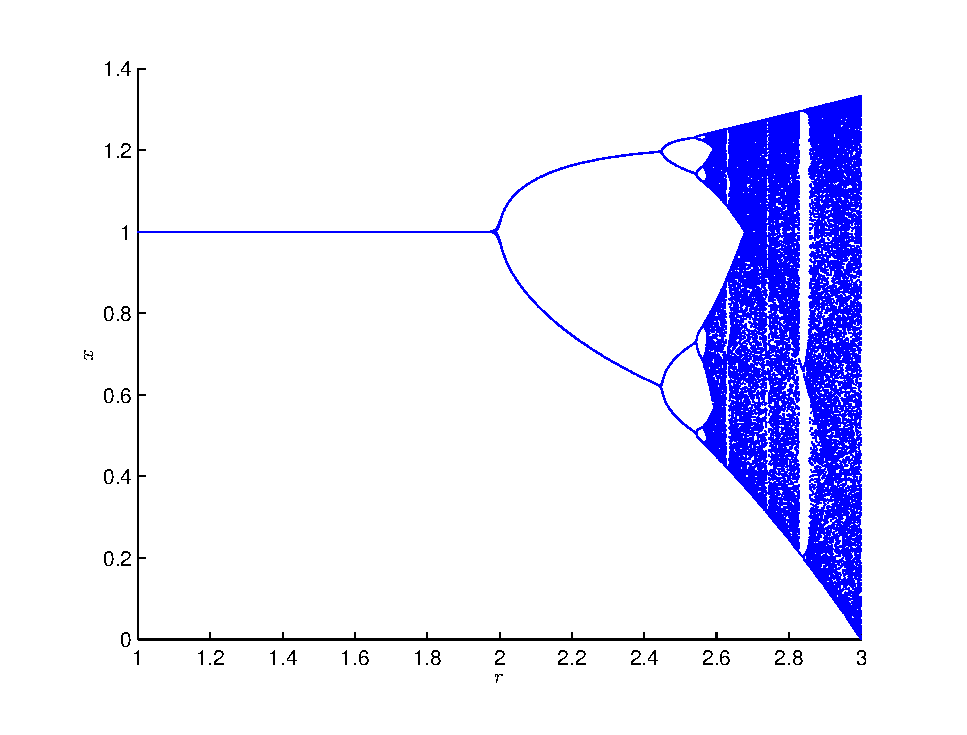
\includegraphics[width=0.7\textwidth]{verhulstbifur}
    \caption{Bifurcation diagram for the Verhulst map}
    \centering
\end{figure}


We will first consider the Verhulst map and its behaviour for $ 0 \leq r < 2.57 $. The map is given by the iterative formula $ x_{k+1} = x_k + rx_k(1-x_k) $, where $ r $ is a fixed parameter. To obtain the bifurcation diagram, we will ignore the first 200 iterations of the map and plot the last 100 for each discrete value of $r$. We require a large number of iterations in order to reach the fixed point, as illustrated by a cobweb plot.

To draw a cobweb plot for any point $ x $, first draw the line $ y = x $ and the curve $ f(x) = x + rx(1-x) $.  Draw a vertical line from either the initial coordinate $ (x_0,0) $ to the curve, obtaining $ (x_0,f(x_0)) $. Then, from this point draw a horizontal line to $ y = x $, giving the point $ (f(x_0),f(x_0)) $. For the next iteration, we repeat this method, with the exception of drawing a vertical line from $ (f(x_0),f(x_0)) $ to the curve instead. Each iteration brings us closer to the fixed point. 


The bifurcation diagram exhibits three stages of behaviour:
\begin{itemize}
\item For $ r < 2 $ the map eventually approaches a stable fixed point of $ x=1 $.

\item At $ r = 2 $ the map undergoes a period doubling bifurcation. We can see in figure (3b) that the map oscillates between two fixed points. This period doubling cascade continues with the number of fixed points doubling until we reach $ r = 2.57 $.

\item For values of $ r > 2.57 $, we observe chaotic behaviour in the map. Graphing $ x $ against the number of iterations
shows there to be no discernible pattern in the oscillations, with $ x $ fluctuating with each iteration. The cobweb plot for $ r = 2.7 $, shown in figure (3c) shows no convergence towards any fixed point.
\end{itemize}

\begin{figure}
    \centering
    \begin{subfigure}[b]{0.3\textwidth}
        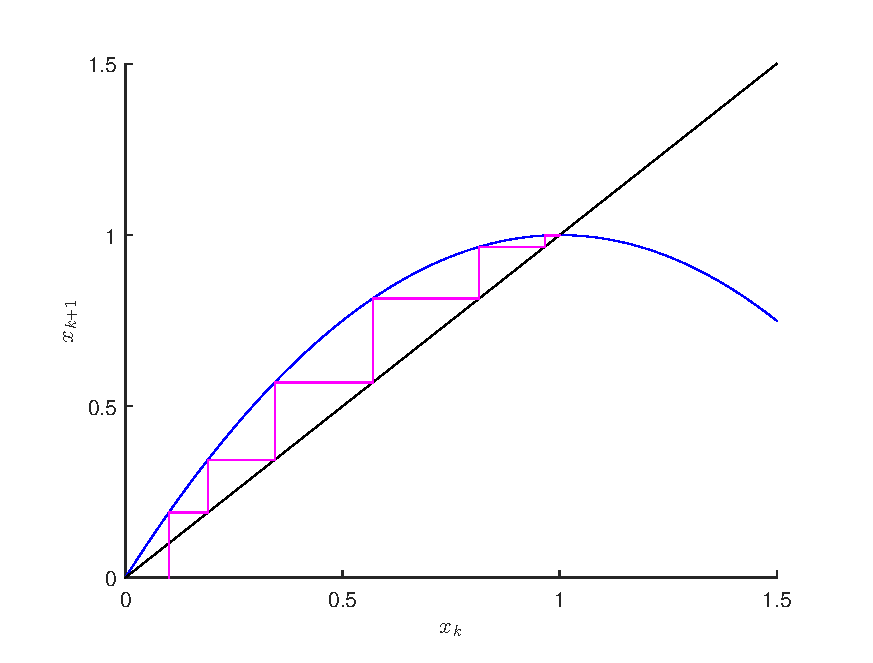
\includegraphics[width=\textwidth]{cobweb1}
        \caption{Cobweb plot for r=1, \\100 iterations}
    \end{subfigure}%
    ~ %add desired spacing between images, e. g. ~, \quad, \qquad etc.
      %(or a blank line to force the subfigure onto a new line)
    \begin{subfigure}[b]{0.3\textwidth}
        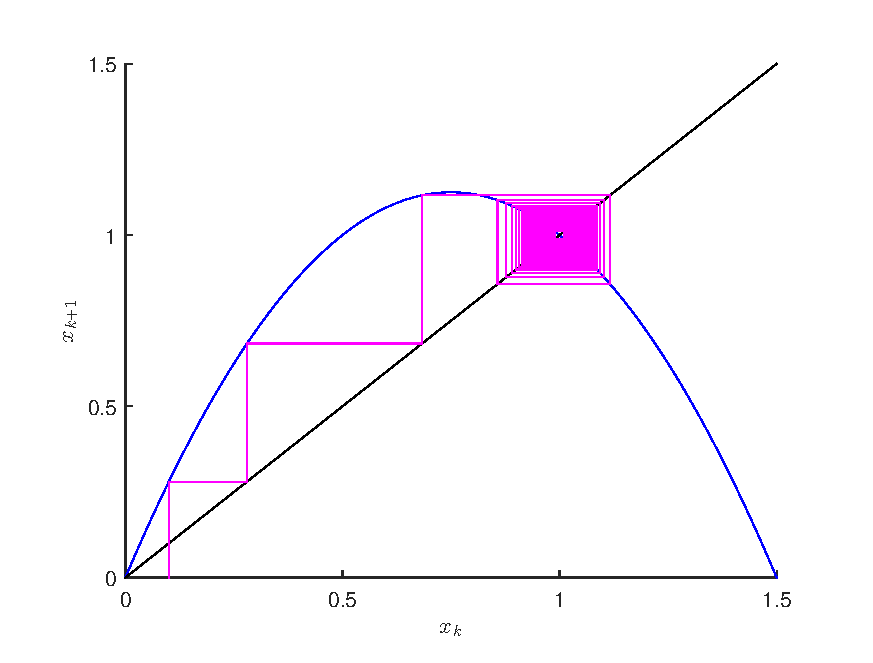
\includegraphics[width=\textwidth]{cobweb2}
        \caption{Cobweb plot for r=2, \\ 1000 iterations}
    \end{subfigure}
    ~ %add desired spacing between images, e. g. ~, \quad, \qquad etc.
      %(or a blank line to force the subfigure onto a new line)
    \begin{subfigure}[b]{0.3\textwidth}
        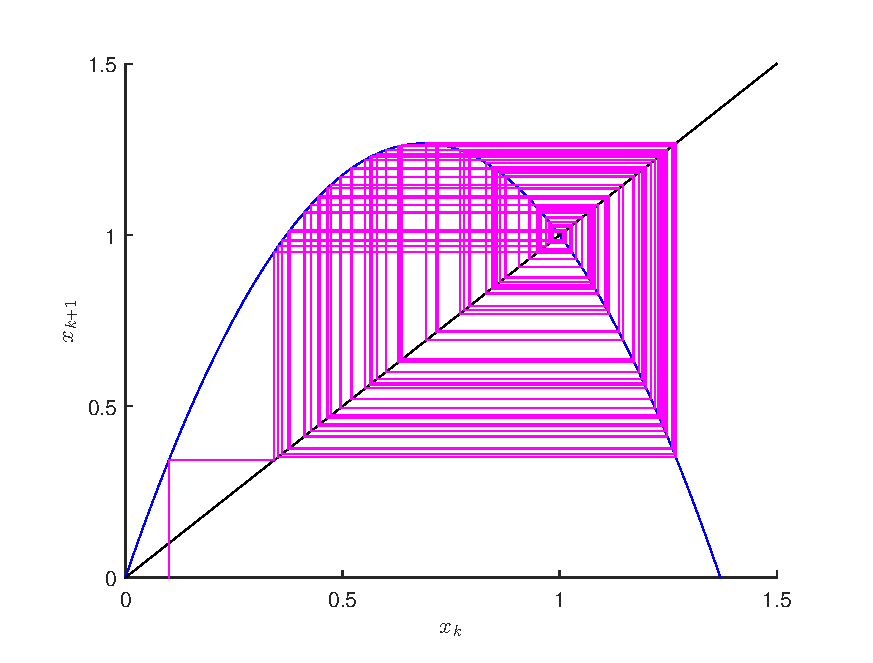
\includegraphics[width=\textwidth]{cobweb3}
        \caption{Cobweb plot for r=2.7, \\100 iterations}
    \end{subfigure}
    \caption{Cobweb plots for the 3 stages of behaviour}\label{fig:animals}
\end{figure} 

\begin{figure}
    \centering
    \begin{subfigure}[b]{0.3\textwidth}
        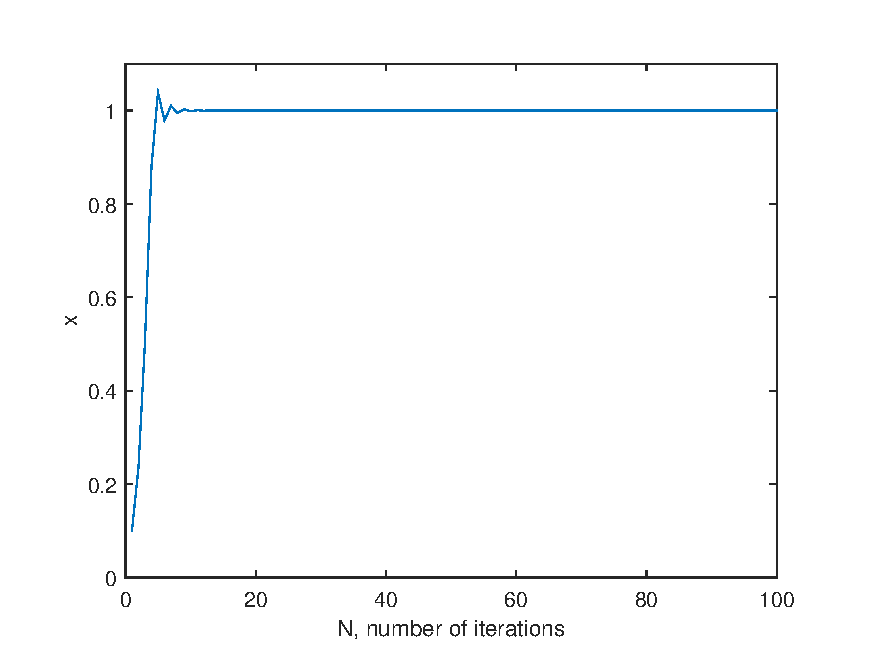
\includegraphics[width=\textwidth]{verhulstPeriod1}
        \caption{r=1, period-1 oscillations}
    \end{subfigure}%
    ~ %add desired spacing between images, e. g. ~, \quad, \qquad etc.
      %(or a blank line to force the subfigure onto a new line)
    \begin{subfigure}[b]{0.3\textwidth}
        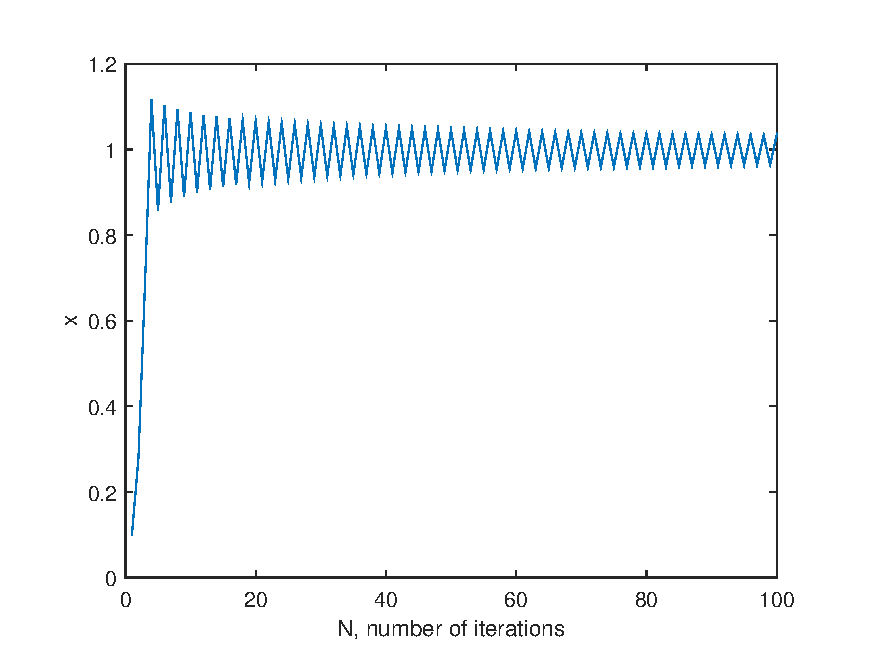
\includegraphics[width=\textwidth]{verhulstPeriod2}
        \caption{r=2, period-2 oscillations}
    \end{subfigure}
    ~ %add desired spacing between images, e. g. ~, \quad, \qquad etc.
      %(or a blank line to force the subfigure onto a new line)
    \begin{subfigure}[b]{0.3\textwidth}
        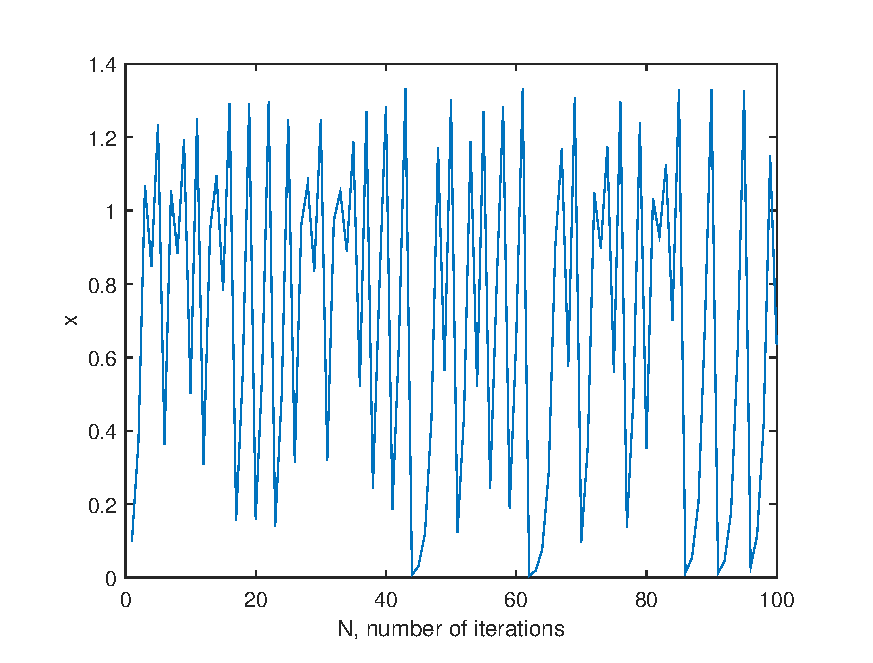
\includegraphics[width=\textwidth]{verhulstChaos}
        \caption{r=4, chaotic region}
    \end{subfigure}
    \caption{Oscillations for the 3 stages of behaviour}\label{fig:animals}
\end{figure} 

The corresponding $ r $ values at the bifurcation points reveal an interesting relationship between the intervals of these neighbouring points. The following formula can be used to obtain the ratios between these intervals:
{\[\frac{r_{n-1} - r_{n-2}}{r_n - r_{n-1}}\] }
where $r_n$ is the corresponding $r$ value for the period-$n$ doubling point. If we take the ratios of the subsequent intervals, we will see that the value eventually converges to 4.669201..., known as the Feigenbaum constant and given by $\delta$ where {\[\delta = \lim_{n \rightarrow \infty} \frac{a_{n-1} - a_{n-2}}{a_n - a_{n-1}}\] } 
where $a_n$ is the value of the bifurcation parameter $a$ at the period-$n$ doubling point. 
Take the first four values of these $ r $ period doubling points as $r_1, r_2, r_3, r_4$. These values were found to be $2.000, 2.450, 2.544, 2.569$ respectively, through inspecting the map at the intervals where the line diverges. We obtain 4.7872 (to 4 decimal places) for the first ratio. However, as our r values are only estimates, they lack the precision necessary to calculate the Feigenbaum constant directly.

Changing the initial value $ x_0 $ does not affect the overall behaviour of the map for the values $ 0 < x_0 < 1 $, as we still observe the same period doubling cascade before reaching chaos when $ r > 2.57 $. While the fixed points remain the same though, the small change in the initial value leads to a slight divergence in the later parts of the map in its chaotic behaviour.​


\section{Other Non-linear Maps}

\subsection{The Logistic and Trigonometric Map}
\begin{figure} [h]
    \centering
    \begin{subfigure}[b]{0.3\textwidth}
        \includegraphics[width=\textwidth]{logisticbifur}
        \caption{Logistic map}
    \end{subfigure}%
    ~ %add desired spacing between images, e. g. ~, \quad, \qquad etc.
      %(or a blank line to force the subfigure onto a new line)
    \begin{subfigure}[b]{0.3\textwidth}
        \includegraphics[width=\textwidth]{+trigbifur}
        \caption{Trigonometric sine map for $x_0>1$}
    \end{subfigure}
    ~ %add desired spacing between images, e. g. ~, \quad, \qquad etc.
      %(or a blank line to force the subfigure onto a new line)
    \begin{subfigure}[b]{0.3\textwidth}
        \includegraphics[width=\textwidth]{-trigbifur}
        \caption{Trigonometric sine map for $x_0<1$}
    \end{subfigure}
    \caption{Bifurcation diagrams}\label{fig:animals}
\end{figure}
For $ k \geq 0$ and for a real, positive parameter, $r$, the Logistic map is defined by the iterative formula $x_{k+1} = rx_k(1-x_k)$ and the trigonometric map by the formula $x_{k+1} = rsinx_k$. Like with the Verhulst map, $k$ takes on discrete values and all three maps involve only a single quantity $x_k$. This distinguishes these three maps as one-dimensional discrete maps.

As with the Verhulst diagram, the logistic and trigonometric maps were constructed with ignoring the initial 200 iterations to stabilize the values of $x$ and produce more accurate images. These images clearly depict moments of period doubling just as the Verhulst map did. The first few succeeding $r$ values for these bifurcation points were calculated as $2.995, 3.448, 3.543, 3.564$ for the logistic map and $1.005, 2.259, 2.616, 2.698$ for the trigonometric map. 

The bifurcation diagrams constructed for the logistic and trigonometric maps have common underlying features and behaviours that were also found in the Verhulst map. Each map initially approached a stable fixed point up until a certain value of $r$. For the logistic and trigonometric map, this value was $r = 3$ and $r =2.259$ respectively. This $r$ value indicated the starting point where a series of period doubling occurs with the interval between the following bifurcation points decreasing as $r$ increased. The ratio of the successive intervals between these points will give the Feigenbaum constant. Further calculations of ratios will attain a greater degree of accuracy. After this series of bifurcation points, the maps exhibited chaotic behaviour just as the Verhulst map did. The corresponding $r$ values in this region for the logistic map was when $r > 3.57$, and when $r > 2.698$ for the trigonometric map.

Examining the chaotic region reveals the fractal properties of the map. If we enlarge certain areas, such as around the point $ r = 3.8 $ on the logistic map and $ r = 3.6 $ on the trigonometric map , we can see that the branch at this point resembles the whole map. In particular, the logistic map has strong connections with the Mandelbrot set as is later explored.

For the logistic map, varying the initial $x$ values within the range of $ 0 < x_0 < 1$ does not change the common features and behaviours of the map, much like we observed in the Verhulst map. However, varying the initial values for $x_0$ can change the image of the trigonometric map. For certain values, the graph can be reflected in the line $x = 0$. This is directly dependent on the sign of $\sin{x}$. For all initial values of $x_0$ such that $\sin{x_0} > 0$, the resultant graphs have no obvious differences. However, for the $x_0$ values where $\sin{x_0} < 0$, the graphs displayed are reflections of the first set of graphs in the line $x = 0$. For values of $x_0$ where $\sin{x_0} = 0$ (i.e when $x_0$ is an integer multiple of $\pi$), the graph at $r \approx 1.15$ shows a sudden jump from $x = 0$ to $x \approx 1$  when $x_0$ is an odd integer multiple of $\pi$ or from $x = 0$ to $x \approx -1$ when it is an even integer multiple. When $x_0 = 0$ the consequent iterated $x$ values all equal to $0$ and so the output of the graph is the line $x = 0$. Despite these initial values of $x_0$ changing the appearance of the graph, the underlying behaviour common to all three maps stay the same for the trigonometric map for all $x_0$ values with the exception of when $x_0 = 0$. 


\subsection{The Tent Map}
The tent map is a single parameter, one-dimensional map defined by the formula :
{ \[ x_{k+1} = \begin{cases}
rx_k      & for\  x_k<\frac{1}{2} \\ 
r(1-x_k)  & for\  \frac{1}{2}\leq x_k\end{cases} \]}
which can be rewritten as $x_{k+1}=r(\frac{1}{2}-\left|(\frac{1}{2}-x)\right|)$. 
It shares many similarities with the other non-linear maps and exhibits the same period doubling to chaos. With the initial condition of $ x=0.1 $, for $ r<1 $, the map converges to the fixed point $ x=0 $. At $ r=1 $, the fixed points converge to $ x=0.1 $. When $ r>1 $, the system oscillates between two fixed points. Thus, the intervals of period bifurcation can also be used to calculate the Feigenbaum constant. 

\begin{wrapfigure}{r}{0.5\textwidth} %this figure will be at the right
    \centering
    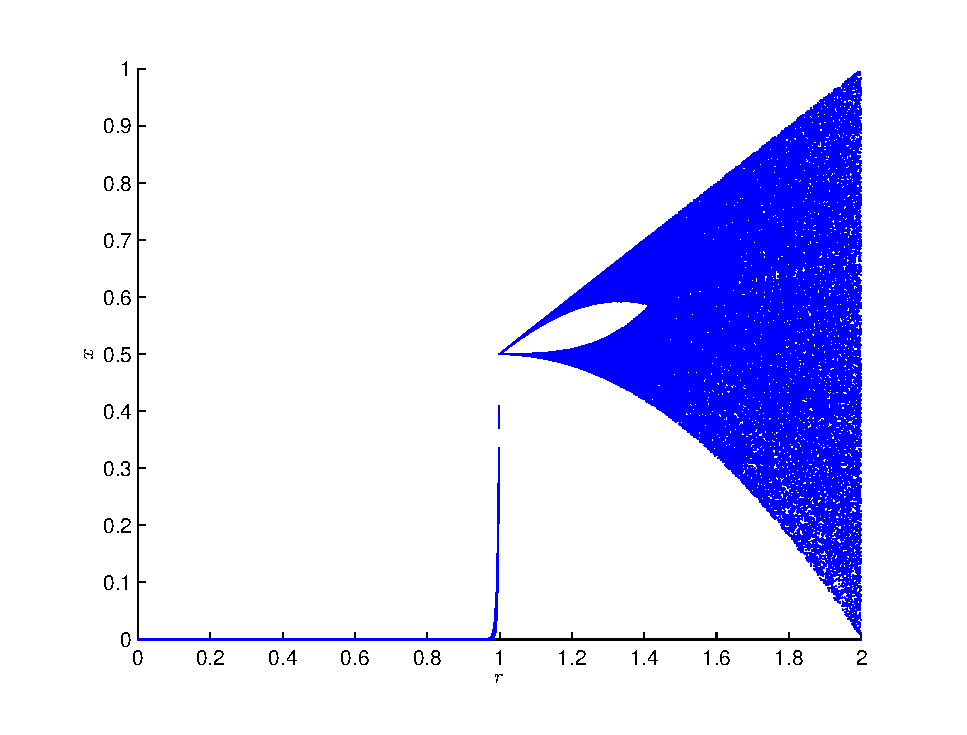
\includegraphics[width=0.5\textwidth]{tentbifur}
    \caption{Bifurcation diagram for the tent map}
\end{wrapfigure}

Similarly to the logistic and Verhulst map, changing the initial value $ x_0 $ within the range of $ 0 < x_0 < 1$ does not affect the overall behaviour and but does change the values of the fixed points. While for $ r<1 $, the map will still converge $ x=0 $ for all initial values, at $ r=1 $, the fixed points will converge to $ x=1-x_0 $. Beyond $ r=1 $, the map descends into chaos with varying fixed points that differ depending on the initial value.

An interesting feature of the tent map is its relationship with the logistic map. Take the logistic map with parameter $ r=4 $ and the tent map with parameter $ r=2 $. 
\\Then  
\\$y_{k+1} = 4y_k(1-x_k)$ 
\\{$x_{k+1} = \begin{cases}
2x_k      & for\  x_k<\frac{1}{2} \\ 
2(1-x_k)  & for\  \frac{1}{2}\leq x_k\end{cases}$}. 
\\By substituting $ x_k=\frac{2}{\pi}sin^-1(\sqrt{y_k})$, we can obtain the logistic map from the tent map.

\subsection{The H{\'e}non Map}
The H{\'e}non map is a two-dimensional map given by the equations with parameters $ a $ and $ b $:
\begin{gather*}
x_{k+1} = 1-ax_k^2+y_k
\\y_{k+1}=bx_k
\end{gather*}
Figure (6a) shows the attractor of the classical map where $ a=1.4 $ and $ b=0.3 $. The attractor possesses fractal properties and is thus a strange attractor; if we magnify any region of the map, shown in figure (6b), we will see that what appears to be a single line from afar is in fact, composed of many lines. 

\begin{figure}[h]
    \centering
    \begin{subfigure}[b]{0.45\textwidth}
        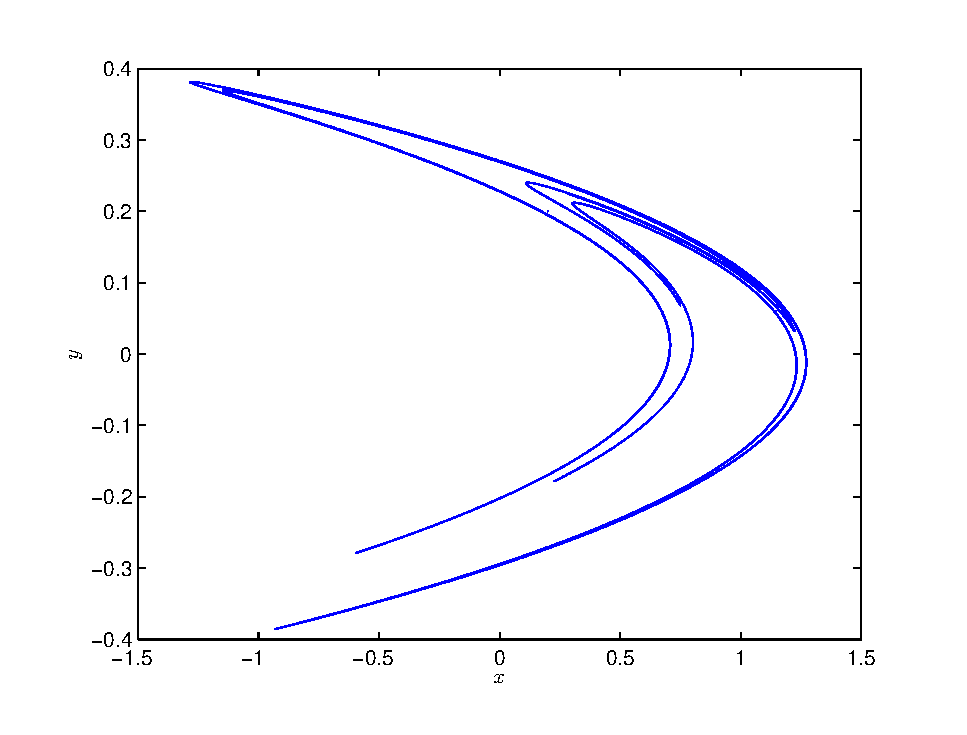
\includegraphics[width=\textwidth]{classicalhenon}
        \caption{Classical h{\'e}non attractor: a=1.4, b=0.3}
        \label{fig:tiger}
    \end{subfigure}
    ~ %add desired spacing between images, e. g. ~, \quad, \qquad etc.
      %(or a blank line to force the subfigure onto a new line)
    \begin{subfigure}[b]{0.45\textwidth}
        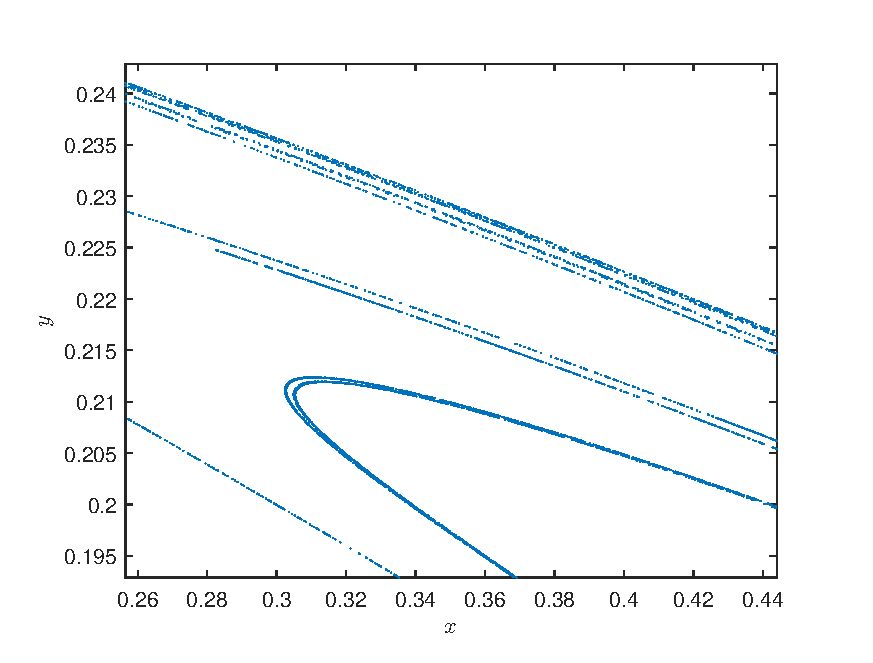
\includegraphics[width=\textwidth]{henoncloseup}
        \caption{Magnification of region on attractor}
        \label{fig:mouse}
    \end{subfigure}
    \caption{H{\'e}non classical attractor}\label{fig:animals}
\end{figure} 
The effect of changing the initial conditions is well illustrated in this map. Some examples are shown in figure 7.  
-1.3
\begin{figure}[h]
    \centering
    \begin{subfigure}[b]{0.45\textwidth}
        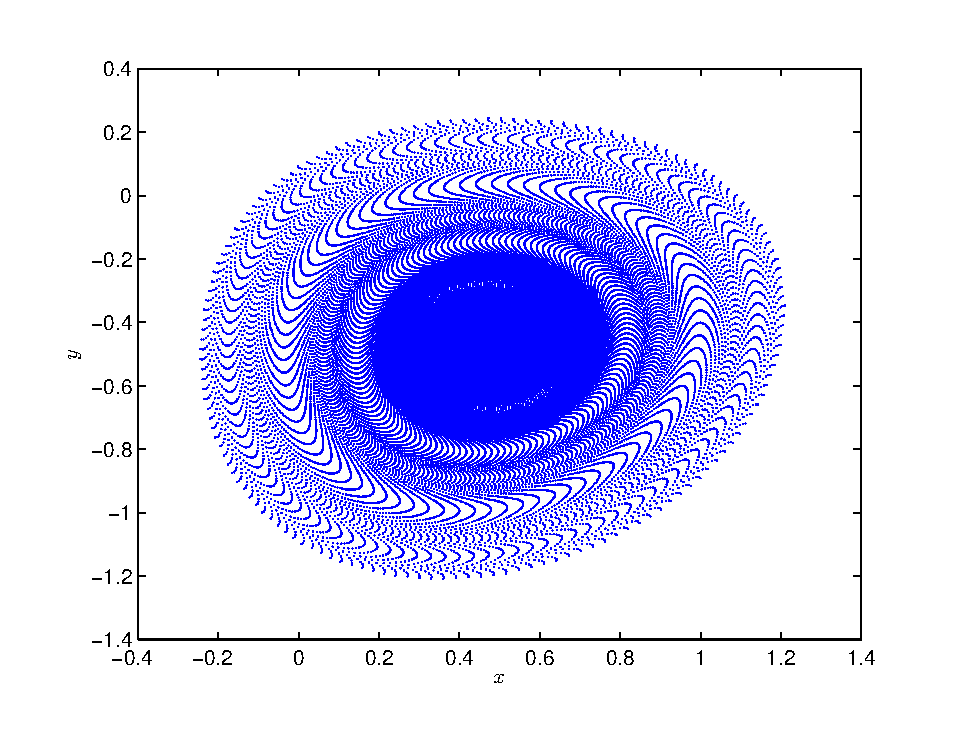
\includegraphics[width=\textwidth]{henon1}
        \caption{a=0.2, b=-0.9999}
        \label{fig:tiger}
    \end{subfigure}
    ~ %add desired spacing between images, e. g. ~, \quad, \qquad etc.
      %(or a blank line to force the subfigure onto a new line)
    \begin{subfigure}[b]{0.45\textwidth}
        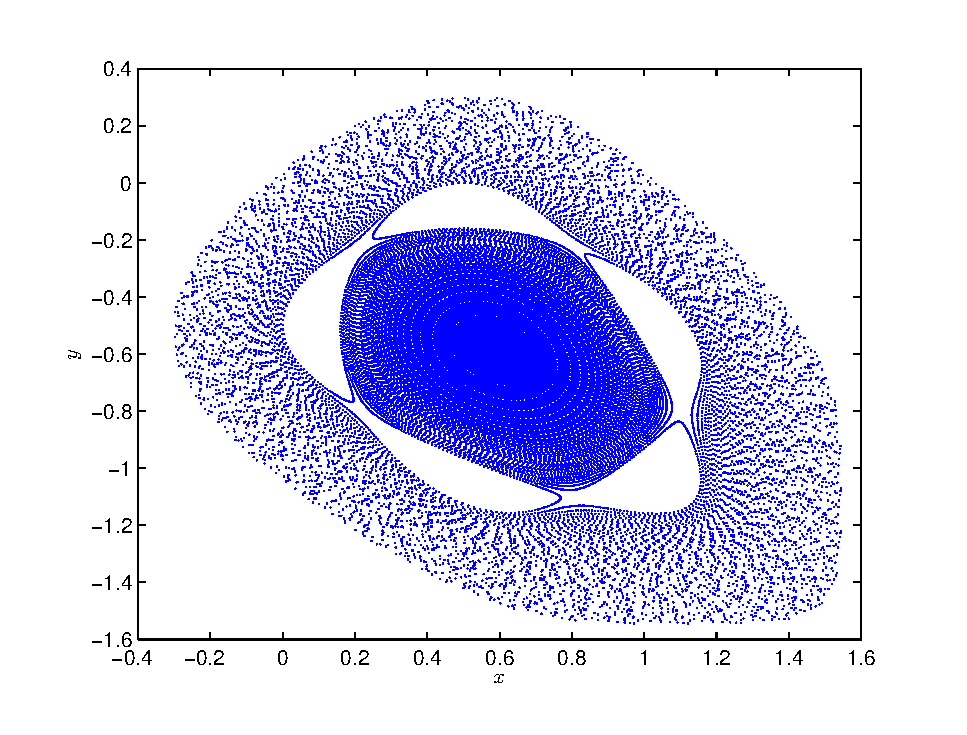
\includegraphics[width=\textwidth]{henon2}
        \caption{a=-0.5, b=-0.9999}
        \label{fig:mouse}
    \end{subfigure}
    \caption{Other H{\'e}non maps}\label{fig:animals}
\end{figure} 

\pagebreak

\begin{wrapfigure}{r}{0.5\textwidth} %this figure will be at the right
    \centering
    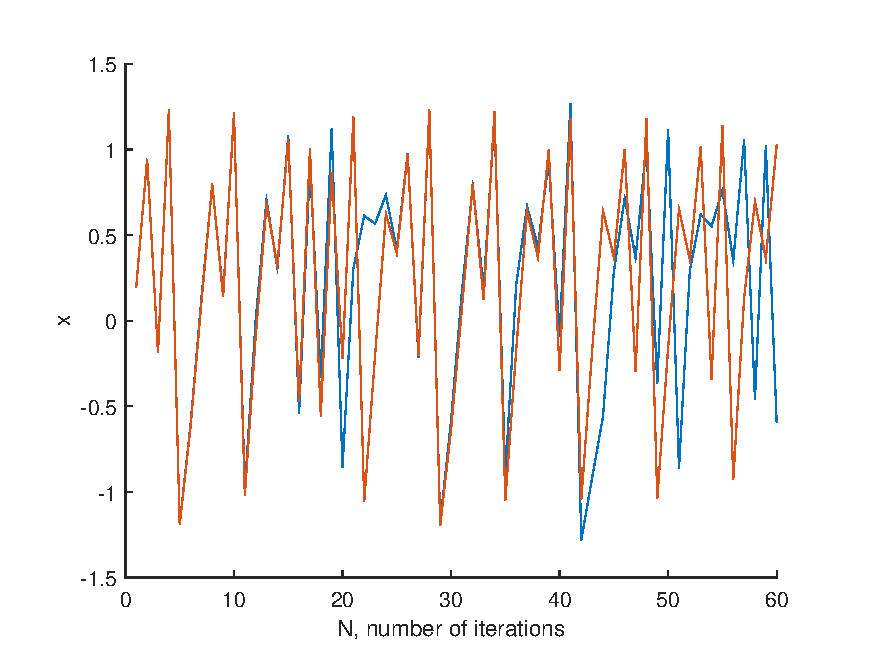
\includegraphics[width=0.42\textwidth]{henonchangingconditions}
    \caption{}
\end{wrapfigure}

The H{\'e}non Map is very sensitive to the initial conditions. Figure 8 demonstrates the quick divergence in the iterations of x after only increasing both $ a $ and $ b $ by 0.01. Small changes in the initial conditions lead to considerable differences in the future behaviour.

The bifurcation diagram for the H{\'e}non map follows the same behaviour as the previous maps. Changing the parameter of b will not change the general shape of the diagram, just as we found with the other maps, so long as we remain within the range $-1<b<1$.
\pagebreak

\section{The Mandelbrot Set}
\subsection{Introduction}
The infinitely complex patterns and self similarity of fractals is an enlightening aspect of mathematics that has intrigued not just mathematicians, but the whole world for centuries, one prime example being the Mandelbrot set. As M.L.Frame once wrote: ``Although the Mandelbrot set is purely a mathematical object, it has fired many imaginations", this has indeed been the case, producing arguably the most ``beautiful of mathematical objects" - utilising the advancement of computer technology in the 1980s- that has inspired even ``philosophers and biologists [to] wonder about the complexity of life itself"~\cite{FractalsGraphics}. As a result, the Mandelbrot set has become one of the most famous computer-generated fractals. It is particularly known not only for its aesthetically pleasing patterns, but also for being an example of an extremely intricate structure arising from the application of a simple rule. 

Formally, the Mandelbrot Set is the set of all complex numbers that do not tend to infinity under the iterative function:
\begin{equation}
f_{c}(z_{k+1}) = (z_{k})^2 + c \mbox{ for all }  z_{k}, \mbox{ $c$} \in \mathbb{C}, \mbox{ $k$} \in \mathbb{N}, \hspace{1pt} z_{0} = 0
\end{equation}
In other words, the Mandelbrot set M is defined:
\[M=\{c \in \mathbb{C} | \lim_{k \to \infty} z_{k} \neq \infty\}\]
By definition M is a compact set: eluding to the fact that the set is bounded, specifically, $\exists M>0$ , $\forall k \in \mathbb{Z^+} \mbox{ s.t. } \left|z_{k}\right|\leq M$; and closed, meaning that the function is continuous at its boundary values.

\begin{figure}[h]
    \centering
    \begin{subfigure}[h]{0.45\textwidth}
        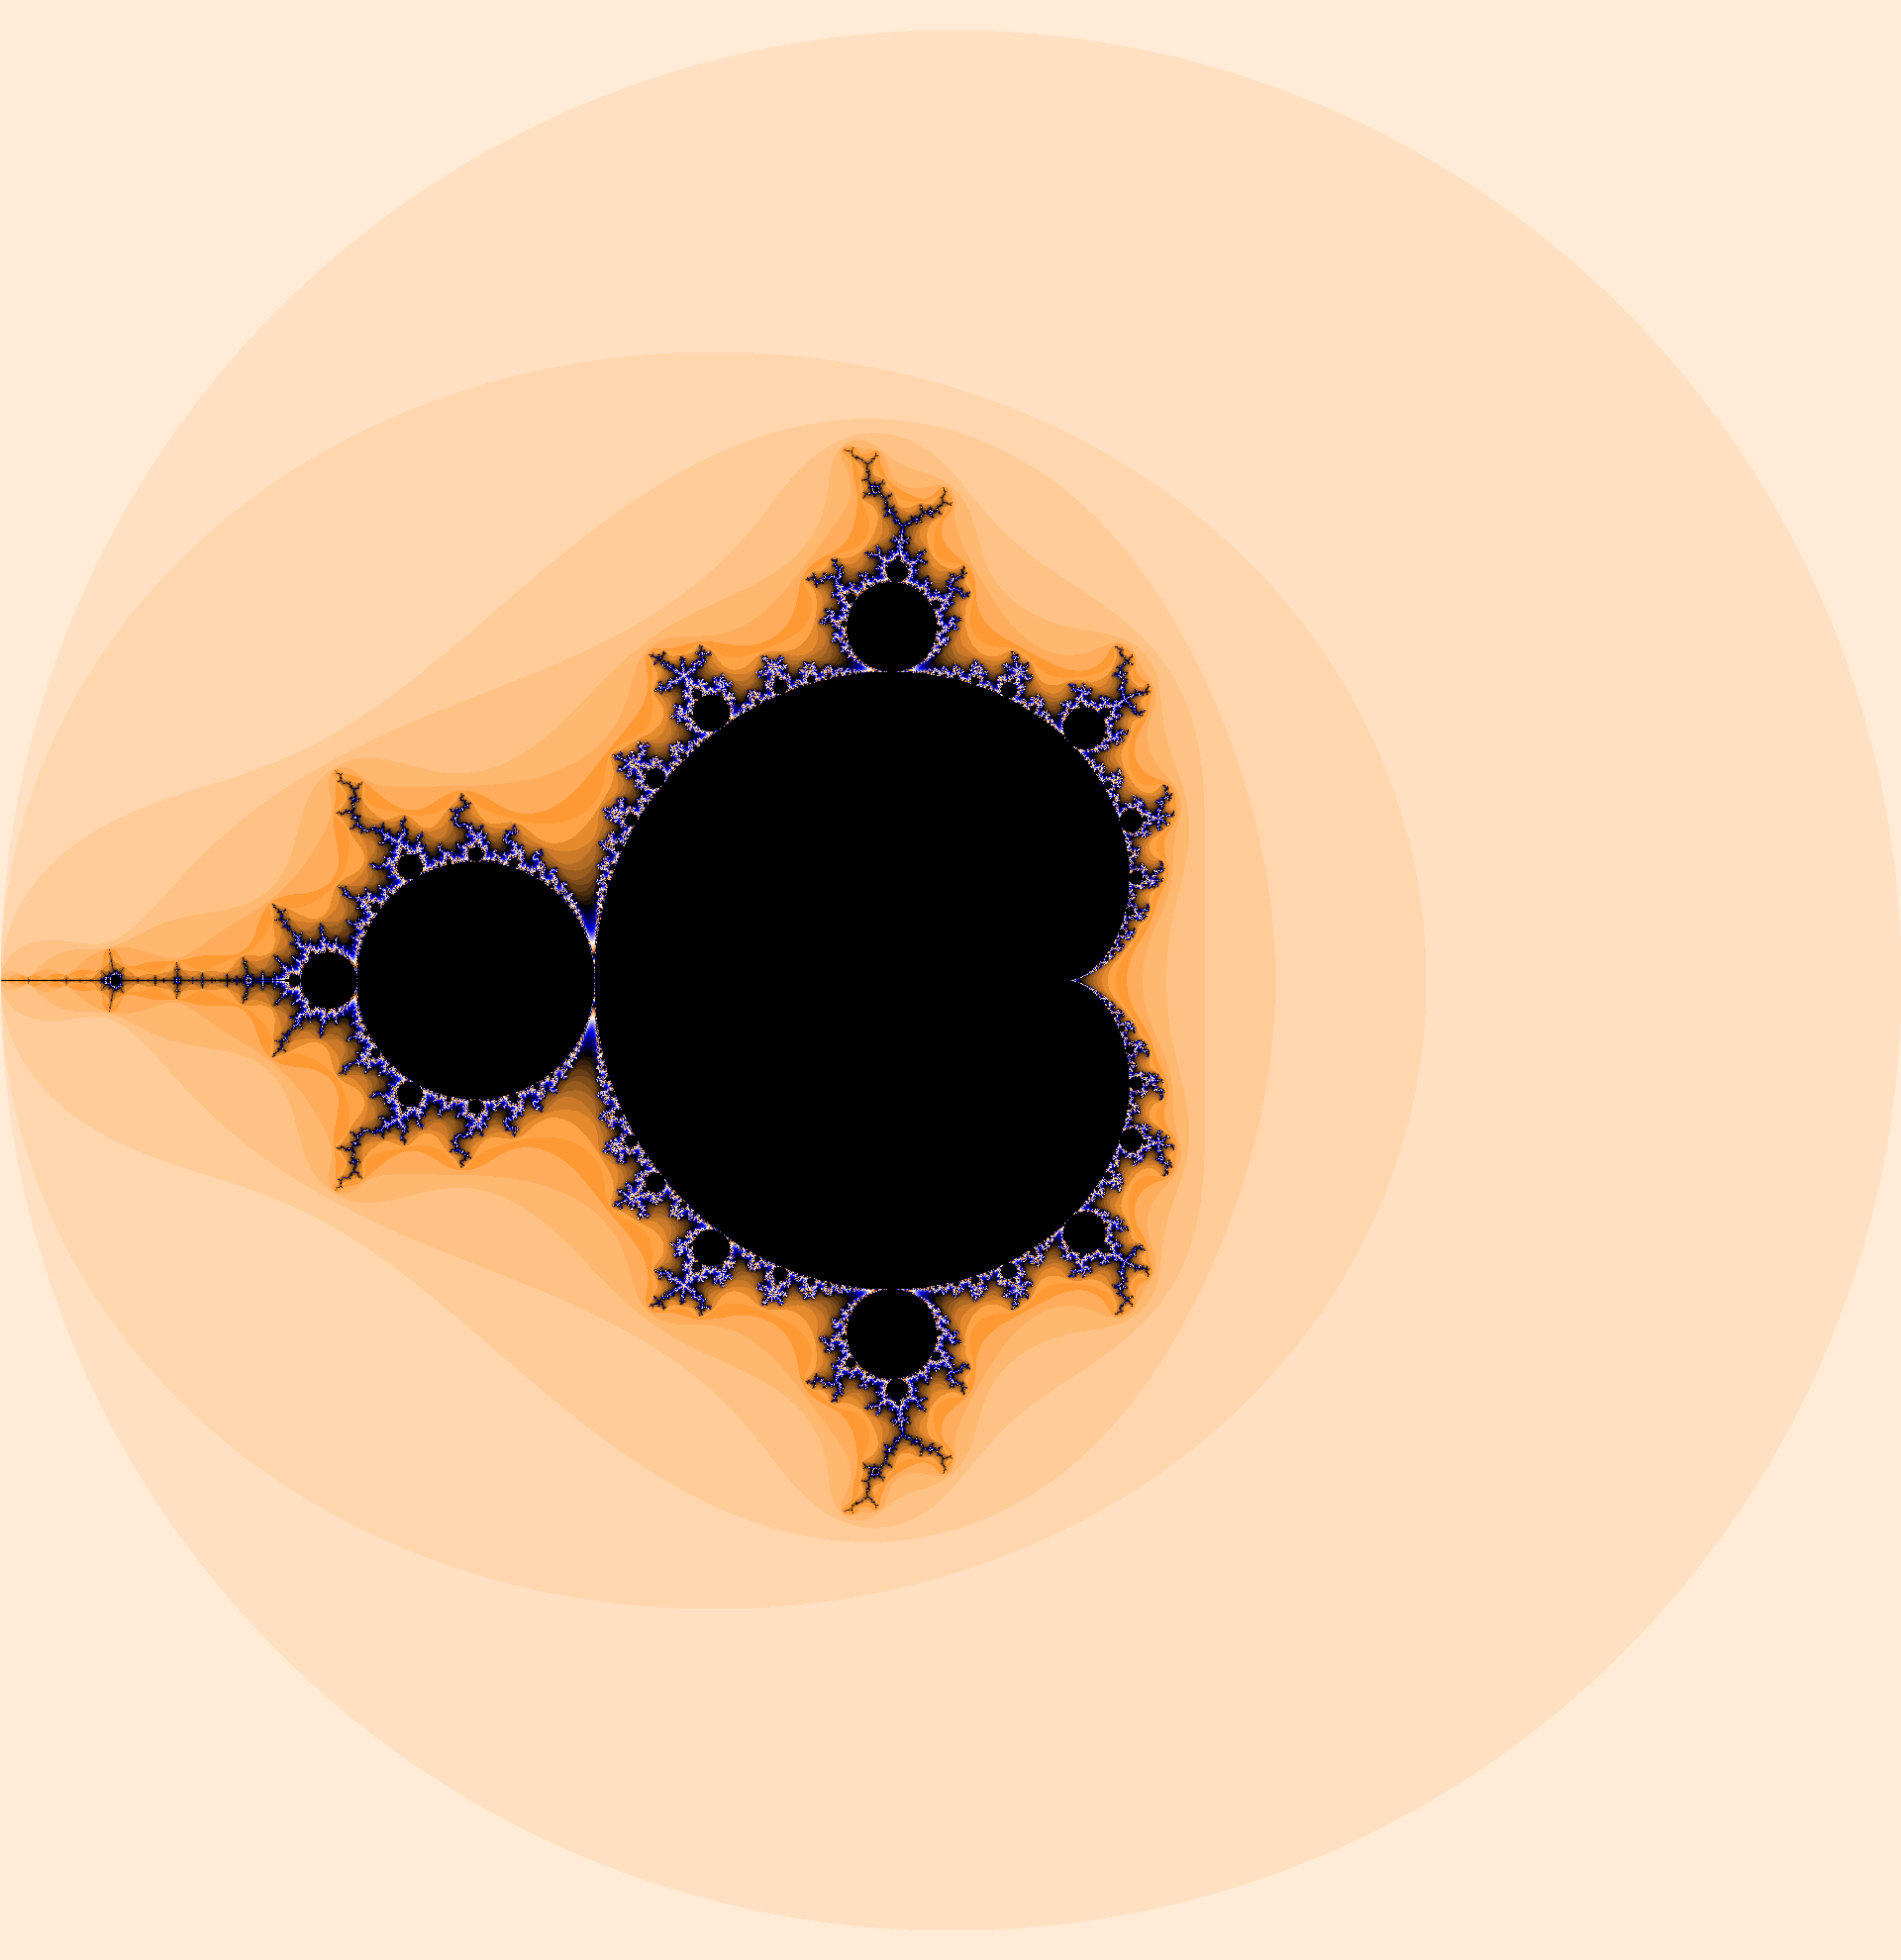
\includegraphics[width=\textwidth]{Morange}
    \end{subfigure}%
    ~ %add desired spacing between images, e. g. ~, \quad, \qquad etc.
      %(or a blank line to force the subfigure onto a new line)
    \begin{subfigure}[h]{0.45\textwidth}
        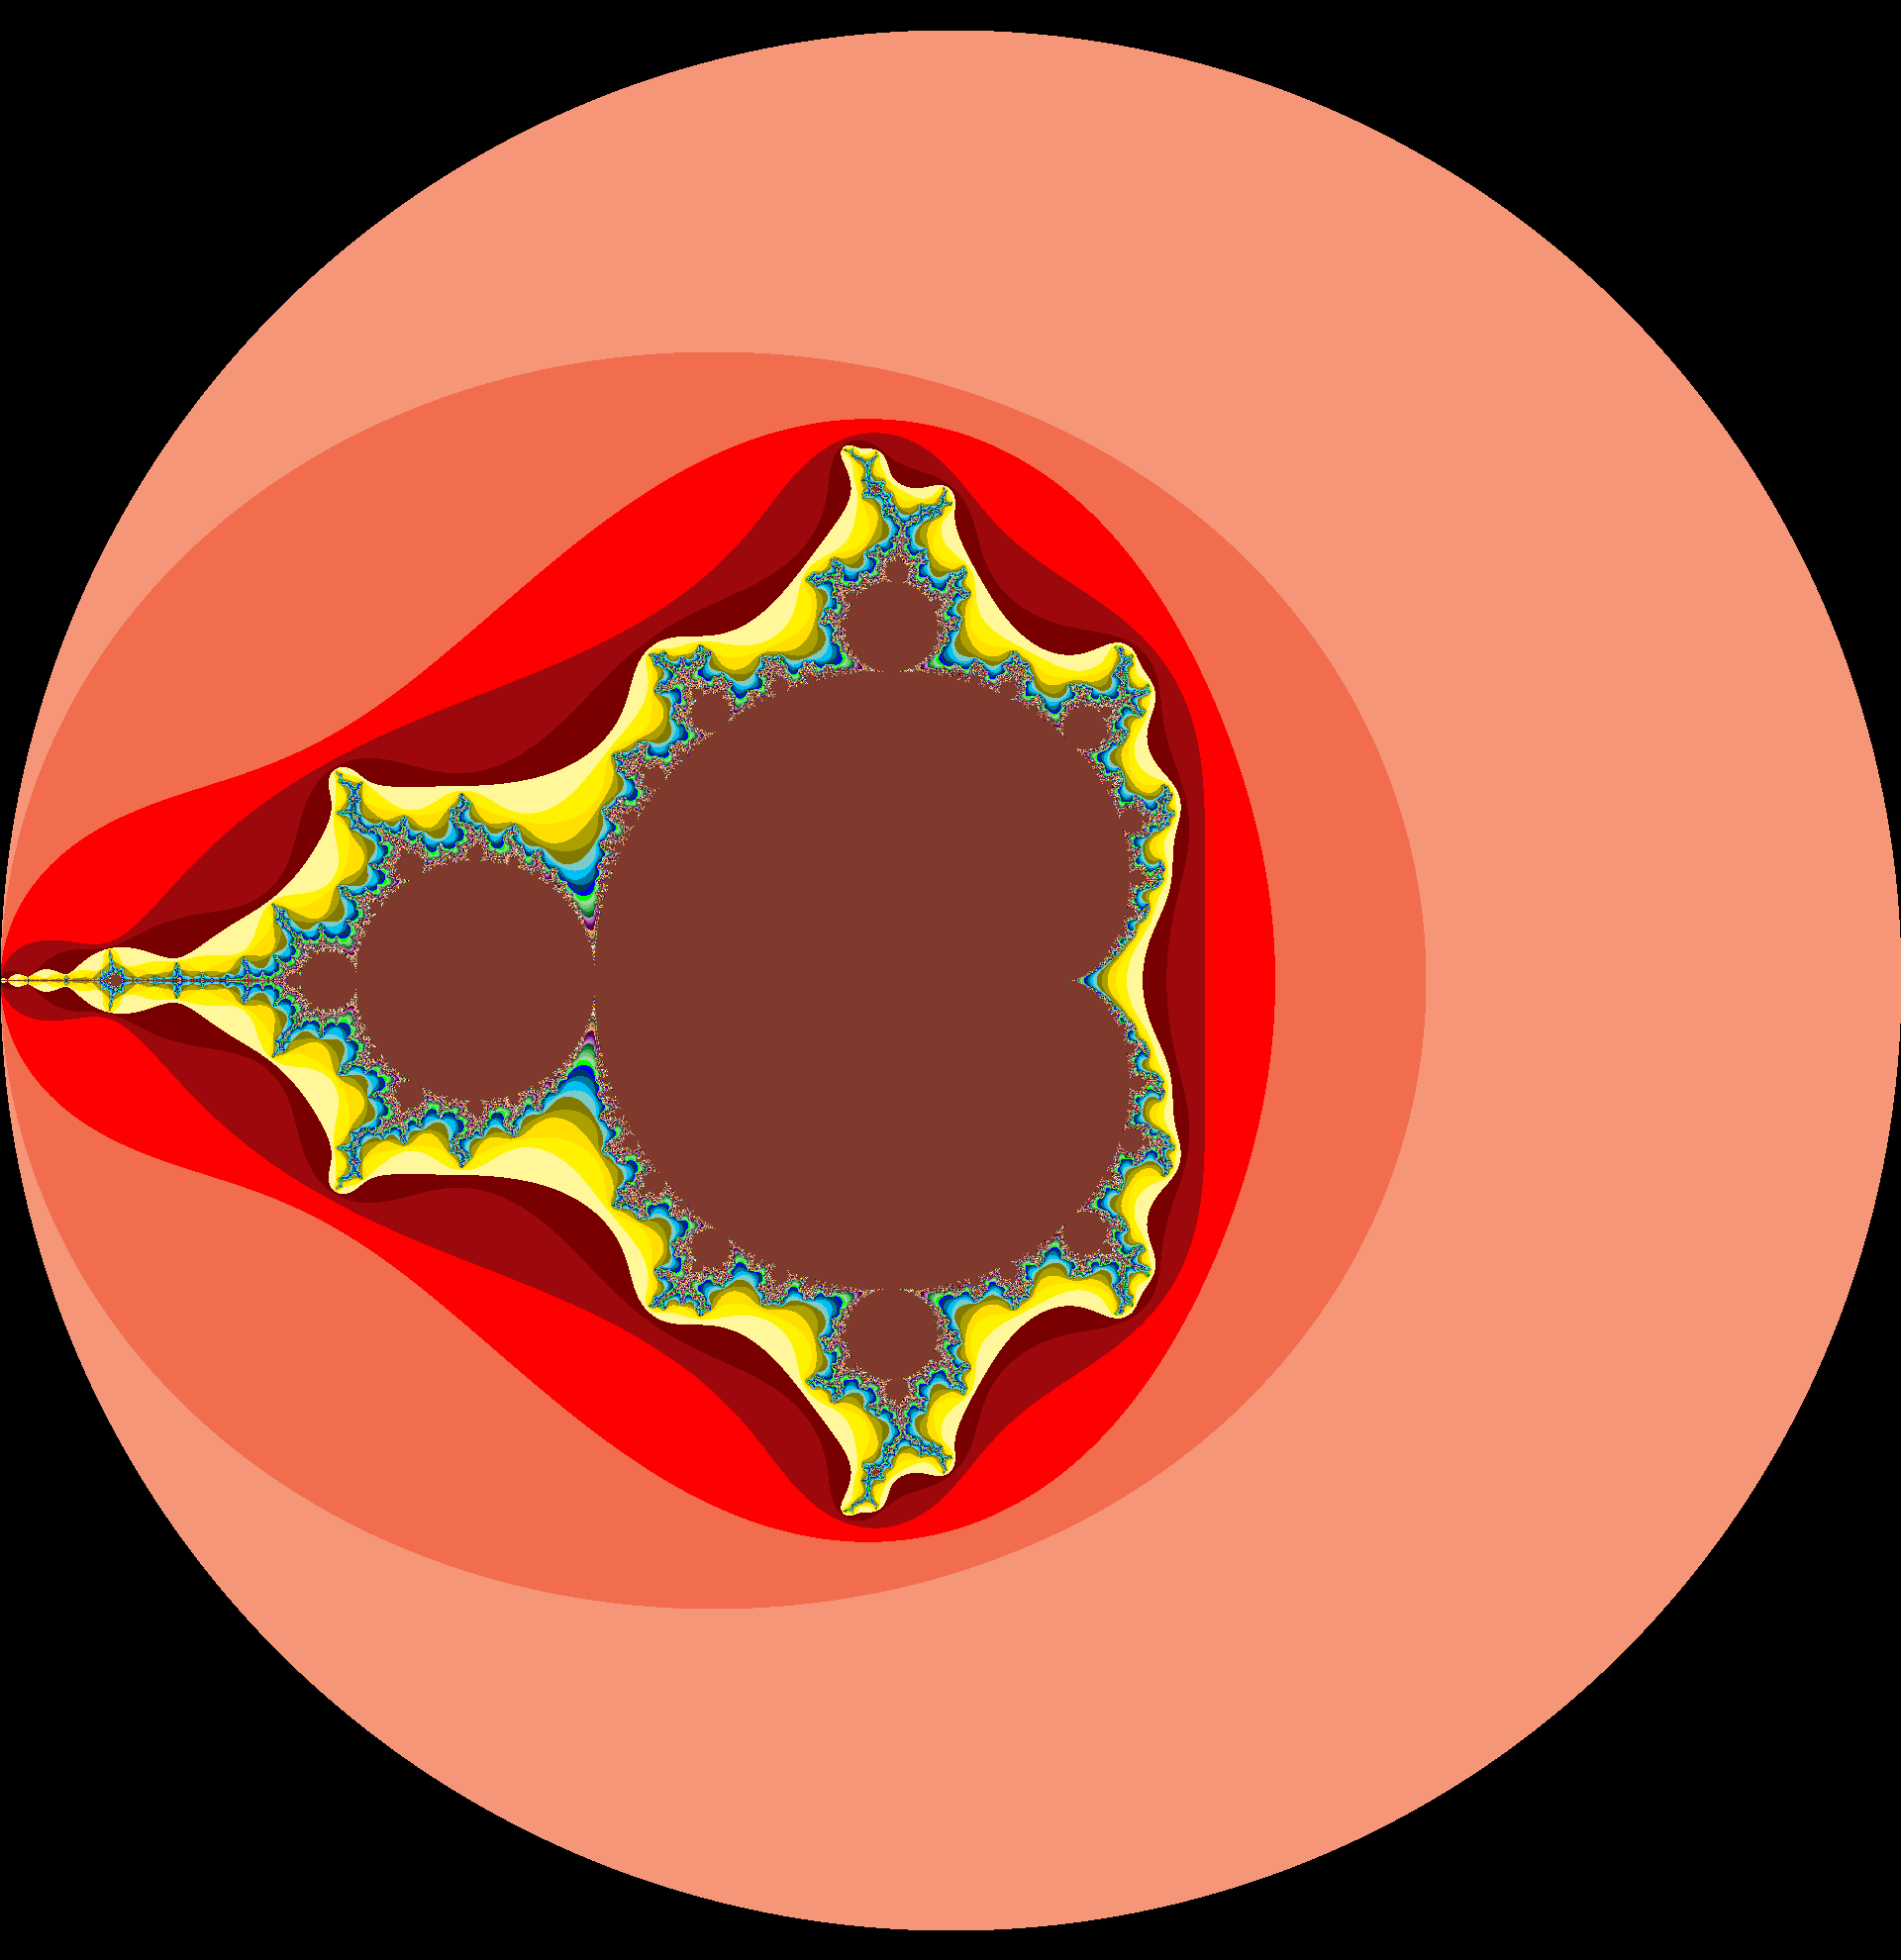
\includegraphics[width=\textwidth]{MandelbrotColoured}
    \end{subfigure}
    ~ %add desired spacing between images, e. g. ~, \quad, \qquad etc.
      %(or a blank line to force the subfigure onto a new line)
    \caption{Mandelbrot sets}\label{fig:MSets}
\end{figure} 

\subsection{At first glance}

Suppose we were to observe the function $y = x^2 + c$ with $x_{0} = 0$ under iteration, with $c$ $\in \mathbb{R}$ and $c$ as an arbitrary constant. Predictably, the process tends to infinity (exponentially) across almost all real values of $c$, however as we approach the region of [-2 ,0.25], we observe a different behaviour. 
Within the region [-2 ,0.25], the iteration does not approach any particular limit, with most values tending to either a single limit, for example $c = 0.25$, or adopting a cyclic behaviour such as $c = -1$, which alternates between results during the iterative process. On the other hand, there are certain values within this range that do not follow this cyclic behaviour, where $c =-1.9$ shows no pattern at all for this orbit; a phenomenon described as chaotic behaviour, as shown in Table 1.


\begin{table}[h]
\parbox{.9\linewidth}{
\centering
\begin{tabular}[h]{||c c c c||} 
        \hline
        Value of c & 0.25 & -1 & -1.9 \\ [0.5ex] 
        \hline\hline
        1st Iteration & 0.3125 & 0 & 1.71 \\ 
        \hline
        2nd Iteration & 0.3477 & -1 & 1.0241 \\
        \hline
        3rd Iteration & 0.3709 & 0 & -0.8512  \\
        \hline
        4th Iteration & 0.3875 & -1 & -1.1754 \\ [1ex]
        \hline
\end{tabular}
\caption{Cycles}
}
\end{table}

Furthermore the process of iteration of $x^2 +c$ where $-2\leq c \leq 0.25$ presents the dichotomy of cyclic, orderly behaviour against chaotic behaviour, and it is this unpredictability of the function under iteration within this interval that is the fundamental basis behind the formation of the Mandelbrot set.

\subsection{Extending to the complex plane}

Now extending $y = x^2 + c$ to the complex plane, the region of $x$ for \textbf{not} escaping to infinity under exponential growth, becomes a circle of radius 2, centred at the origin - as shown below:

\textbf{Proof of Escape Criterion: }

Suppose that $|c|>2$ then the first few iterations for the function $h$ are $h(0)=c$, $h(c)=c^2+c$. 
say we were to treat the output of the first iteration $z_{0}$ so $|z_{0}| \geq |c| > 2$, using the triangle inequality we obtain the expression $|z_{0}^2 + c| + |-c| \geq |z_{0}^2|$ and thus: 
\begin{align*}
|z_{0}^2 + c| & \geq |z_{0}|^2 -|c| \mbox{ (by rearranging)}\\
          & \geq |z_{0}|^2 -|z_{0}| \mbox{ (as } |z_{0}| \geq |c| \mbox{)}\\
          & = |z_{0}|(|z_{0}|-1) \mbox{ (by Distribution Law)}\\
          & = |z_{0}|\lambda_{0} \mbox{ where } \lambda_{0}=|z_{0}|-1>1 \mbox{ (since } |z_{0}| > 2 \mbox{)}
\end{align*}

Each iteration results in multiplying the previous result by $\lambda_{0}$, which implies $|z_{1}|>|z_{0}|>2$. Continuing this process produces $|z_{2}|>|z_{0}|\lambda_{0}^2$. Hence $\lambda_{n}=|z_{n}|-1$, and for $n>m$, $\lambda_{n}>\lambda_{m}$. 
By mathematical induction, we have $|z_{n}|>\lambda_{0}^{n}|z_{0}|$. The right hand side tends to infinity with $n$ because $\lambda_{0}>1$, therefore $|z_{n}|$ tends to infinity. $\blacksquare$ \cite{Klebanoff}

Treating the real and imaginary parts of each number as image coordinates, in our implementation of Mandel.java program, pixels are coloured according to how rapidly the sequence diverges. With each iteration, progressively more values of $c$ are excluded from the Mandelbrot set. Thus each progressive colour towards the centre of the Mandelbrot set represents the numbers excluded at a given iteration. The resulting diagram forms the convoluted, web like structure we see in Figure 8. No section of the boundary of the Mandelbrot set is smooth, thus encapsulating the words of the man himself, ``Clouds are not spheres, mountains are not cones, coastlines are not circles, and bark is not smooth, nor does lightning travel in a straight line"~\cite{FractalsGeometry}.

\pagebreak

\subsection{$\pi$ in the Mandelbrot Set}

In 1991, Dave Boll attempted to verify the point (-0.75,0) as infinitely thin, or in other words, that it \emph{connects} the cardioid to the 2-cycle disk. At the time Dave Boll calculated the amount of iterations required for small values of $\epsilon$ belonging to the point $(-0.75,\epsilon)$ to be excluded from the Mandelbrot set. As is apparent in Table 4, $\epsilon \times n_{c} \rightarrow \pi$ as $\epsilon \rightarrow 0$. The symmetry of the Mandelbrot set also ensures that the point $(-0.75, -\epsilon)$ will produce the same result. Another point that draws similar attention is $(0.25+\epsilon, 0)$ where $\sqrt{\epsilon} \times n_{c} \rightarrow \pi$ as $\epsilon \rightarrow 0$. Based on these two points that are referred to as the `neck' and `butt' of the Mandelbrot set respectively, we can attempt to find more points that replicate similar behaviour. Upon further research we found that $(-1.25 - \epsilon ^ 2, \epsilon)$ is another special point and this is located at the boundary of the 2-cycle and 4-cycle disks~\cite{piInMandel}. In this particular case, $2 \times n_{c} \times \epsilon \rightarrow \pi$ as $\epsilon \rightarrow 0$

\begin{table}[h]
\parbox{.4\linewidth}{
\centering
\begin{tabular}[h]{||c c c||} 
	    \hline
        Value of $\epsilon$ & \# of iterations $n_{c}$ & $n_{c} \times \epsilon^{1/2}$ \\ [0.5ex] 
        \hline\hline
        1 & 2 & 2 \\ 
        \hline
        $2^{-5}$ & 16 & 2.828 \\
        \hline
        $2^{-10}$ & 99 & 3.093  \\
        \hline
        $2^{-15}$ & 567 & 3.132  \\ 
        \hline
        $2^{-20}$ & 3215 & 3.139 \\
        \hline
        $2^{-25}$ & 18196 & 3.141 \\ [1ex] 
        \hline
\end{tabular}
\caption{Point (0.25+$\epsilon$, 0)}
}
\hspace{1.5cm}
\parbox{.4\linewidth}{
\begin{tabular}[h]{||c c c||} 
        \hline
        Value of $\epsilon$ & \# of iterations $n_{c}$ & $n_{c} \times 2 \times \epsilon$ \\ [0.5ex] 
        \hline\hline
        1 & 1 & 2 \\ 
        \hline
        $10^{-1}$ & 18 & 3.6  \\
        \hline
        $10^{-2}$ & 159 & 3.18  \\
        \hline
        $10^{-3}$ & 1586 & 3.172  \\ 
        \hline
        $10^{-4}$ & 15731 & 3.1462 \\
        \hline
        $10^{-5}$ & 157085 & 3.1417 \\ [1ex] 
        \hline
\end{tabular}
\caption{Point (-1.25 - $\epsilon^2$, $\epsilon$)}
}
\end{table}

\begin{table}[h]
\centering
\begin{tabular}[h]{||c c c||} 
        \hline
        Value of $\epsilon$ & \# of iterations $n_{c}$ & $n_{c} \times \epsilon$ \\ [0.5ex] 
        \hline\hline
        1 & 3 & 3 \\ 
        \hline
        $2^{-5}$ & 101 & 3.15625 \\
        \hline
        $2^{-10}$ & 3217 & 3.14160  \\
        \hline
        $2^{-15}$ & 102945 & 3.14163 \\ [1ex]
        \hline
\end{tabular}
\caption{Point (-0.75, 0+$\epsilon$)}
\end{table}

\subsection{Period doubling cascade}
The term 'Period doubling cascade' - a revelation discovered in the 1970s by Mitchell Feigenbaum, Pierre Coulette and Charels Tresser - refers to how the Mandelbrot set represents the cyclic behaviour of the numbers within the complex set, exhibiting a close relationship with the logistic map curve.

In our figure, the main cardioid of the Mandelbrot set (representing the subset of numbers that converge to one attracting point) is attached at a point to a smaller section, consisting of the parameters for the 2-cycle property. This in turn, is connected to another smaller section of the Mandelbrot set representing the 4-cycle set. As we traverse the real axis further, we see that each adjoining -increasingly smaller- section of the Mandelbrot set represents the complex numbers of cycles double that of the previous section. 

This doubling, cascading behaviour is mirrored by the logistic map, which is shown by the bifurcation diagram in Figure(~\ref{fig:bifurcationgraph}). The intersections of the Mandelbrot set with the real axis are precisely the points that correspond to the bifurcation diagram, where the graph branches off, thus referring to a higher cascade section of the Mandelbrot set. Here we see that the single curve, of the Bifurcation Diagram refers to the one-cycle behaviour of the main cardioid, the branching off into two represents the second bulb, the section of 4 branches refers to the next bulb, and so on. Furthermore the chaotic areas of the Mandelbrot set are reflected by the density of the lines, whereas sparse areas reflect the regions where baby Mandelbrot sets are located.

\begin{figure}[h]
\centering
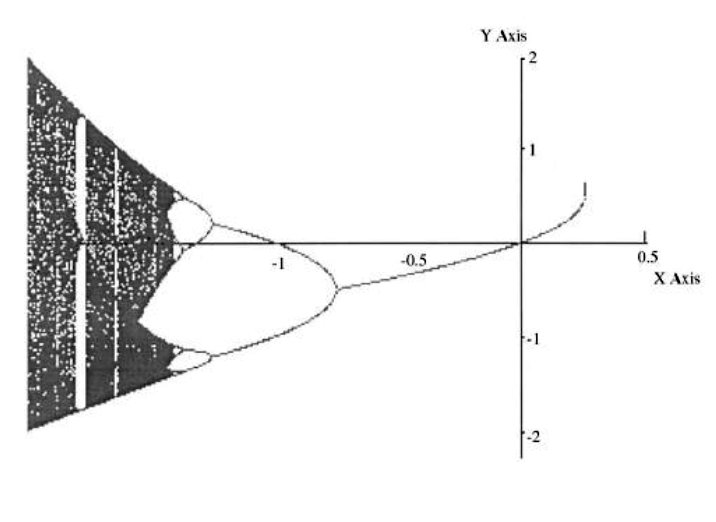
\includegraphics[width=0.65\textwidth]{bifurcationgraph}
\caption{\label{fig:bifurcationgraph}Bifurcation Diagram~\cite{PeriodDoublingBifurcation}}
\end{figure}
\pagebreak
\section{Julia Sets}

The Julia set J is defined:
\[J=\{c \in \mathbb{C} | \lim_{n \to \infty} z_{n} \neq \infty\}\]
where:
\begin{equation}
g_{c}(z_{n+1}) = (z_{n})^2 + K \mbox{ for all }  z_{n}, \mbox{ $K$} \in \mathbb{C}, \mbox{ $n$} \in \mathbb{N}, \hspace{1pt} z_{0} = c 
\end{equation}

Notably, the mathematical definition of the set is almost identical to that of the Mandelbrot set, exhibiting a close relationship between the value of K and the Mandelbrot Set: 

\begin{itemize}
\item If K is inside the Mandelbrot set, the corresponding Julia set for K will be connected, always showing a path from one point in the set to another, as shown in Figure 10(c). 

\item However, even if K is inside the Mandelbrot set there is some variation in the resulting Julia sets based on whether the value of K is close to the border or far away from it: values of K close to the border of the Mandelbrot set result in a “thinner” and “curlier” Julia set, as shown in Figure 11; whereas more centred values of K produce a “thicker” Julia set, as shown in Figure 10(c). 

\item Values of K outside the Mandelbrot set result in a disconnected Julia set, producing an image of at least two “islands”. One possible way of optimising the code used to generate the Mandelbrot set is to make use of the connected property in order to speed up calculations. However, this optimisation would not be able to generate Julia sets because they can be either connected or disconnected. 

\end{itemize}

\noindent Interestingly, despite there being only one Mandelbrot set, there is a contrastingly infinite amount of Julia sets, where each point of the Mandelbrot set corresponds to a unique Julia set.

\subsection{Julia Extension}
Notably, the Julia set produced by the iterative function $z^2 + K, \forall K \in \mathbb{C}$ has a rotational symmetry of 2, indeed it is the case that as the power of $z$ increases, so too does the rotational symmetry of the corresponding Julia set, as shown below.

\begin{figure}[h]
    \centering
    \begin{subfigure}[h]{0.25\textwidth}
        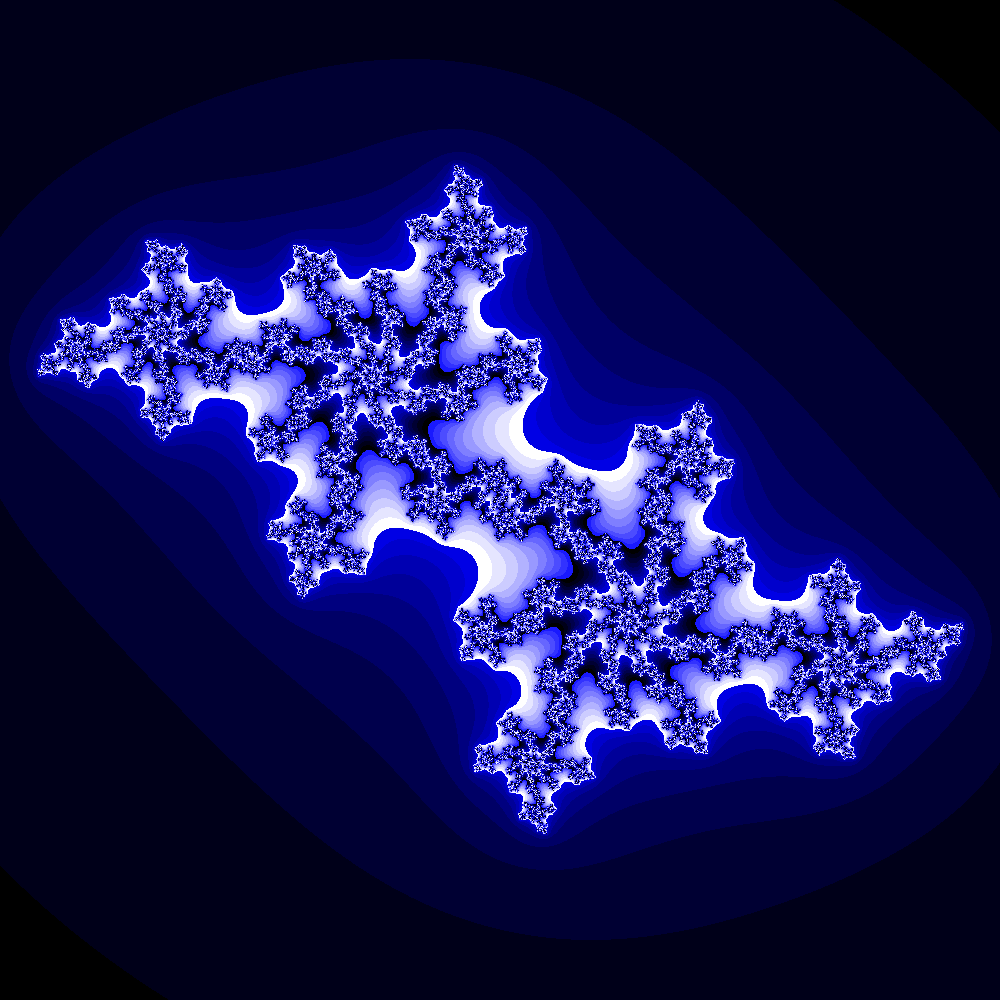
\includegraphics[width=\textwidth]{Julia(1)}
        \caption{K = (-0.4,0.65)}
        \label{fig:gull}
    \end{subfigure}%
    ~ %add desired spacing between images, e. g. ~, \quad, \qquad etc.
      %(or a blank line to force the subfigure onto a new line)
    \begin{subfigure}[h]{0.25\textwidth}
        
\includegraphics[width=\textwidth]{Julia(2)}
        \caption{K =  (0.285,0.01)}
        \label{fig:tiger}
    \end{subfigure}
    ~ %add desired spacing between images, e. g. ~, \quad, \qquad etc.
      %(or a blank line to force the subfigure onto a new line)
    \begin{subfigure}[h]{0.25\textwidth}
        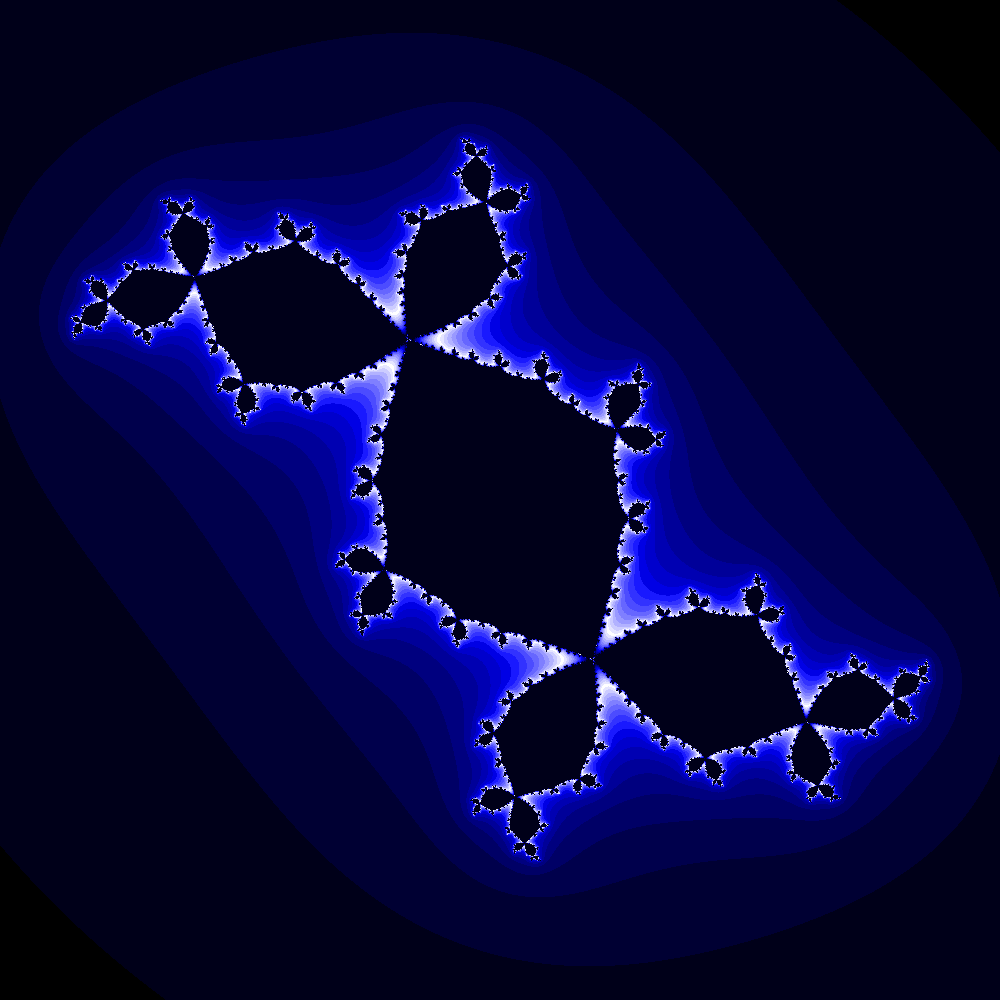
\includegraphics[width=\textwidth]{JuliaRabbit}
        \caption{Douady's Rabbit Fractal}
        \label{fig:mouse}
    \end{subfigure}
    \caption{Julia Sets}\label{fig:animals}
\end{figure} 

\begin{figure}[h]
    \centering
    \begin{subfigure}[h]{0.25\textwidth}
        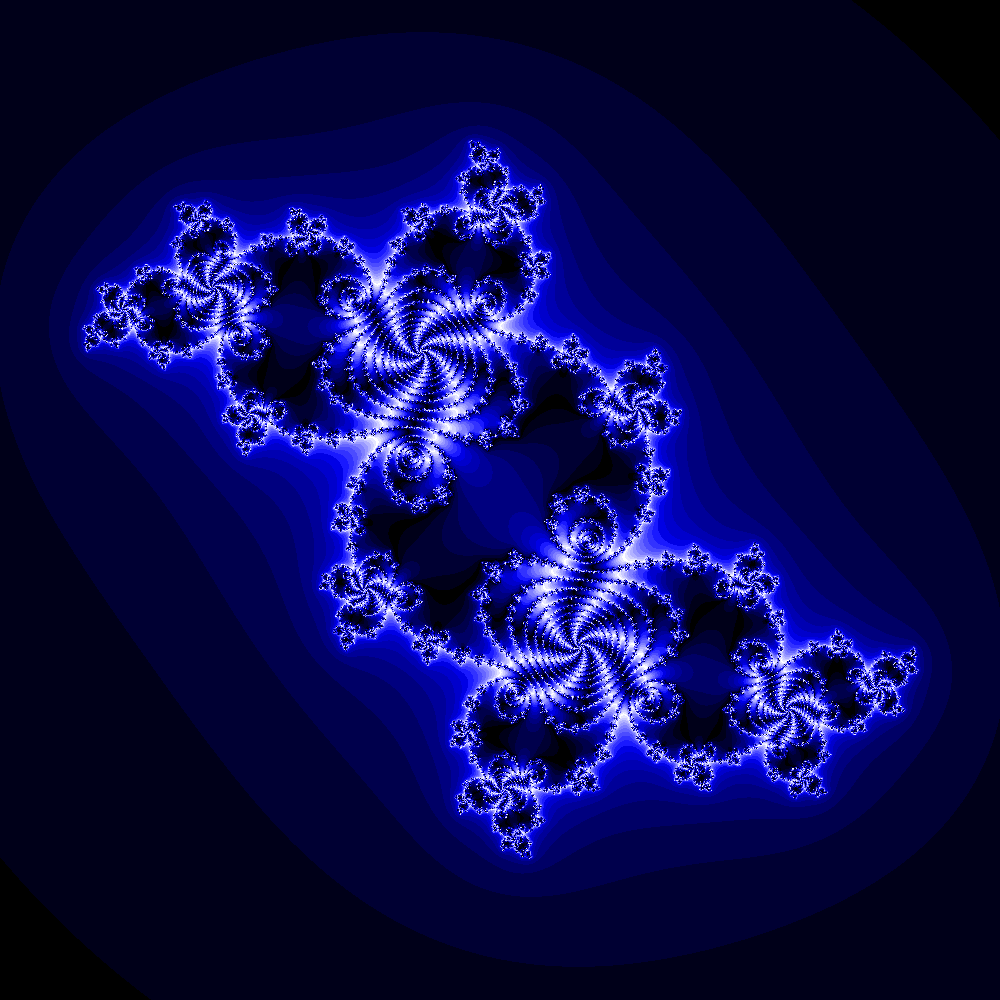
\includegraphics[width=\textwidth]{Julia(3)}
        \caption{K = (-0.1,0.651)}
        \label{fig:gull}
    \end{subfigure}%
    ~ %add desired spacing between images, e. g. ~, \quad, \qquad etc.
      %(or a blank line to force the subfigure onto a new line)
    \begin{subfigure}[h]{0.25\textwidth}
        
\includegraphics[width=\textwidth]{Julia(4)}
        \caption{K = (0.285,0.01)}
        \label{fig:tiger}
    \end{subfigure}
    ~ %add desired spacing between images, e. g. ~, \quad, \qquad etc.
      %(or a blank line to force the subfigure onto a new line)
    \begin{subfigure}[h]{0.25\textwidth}
        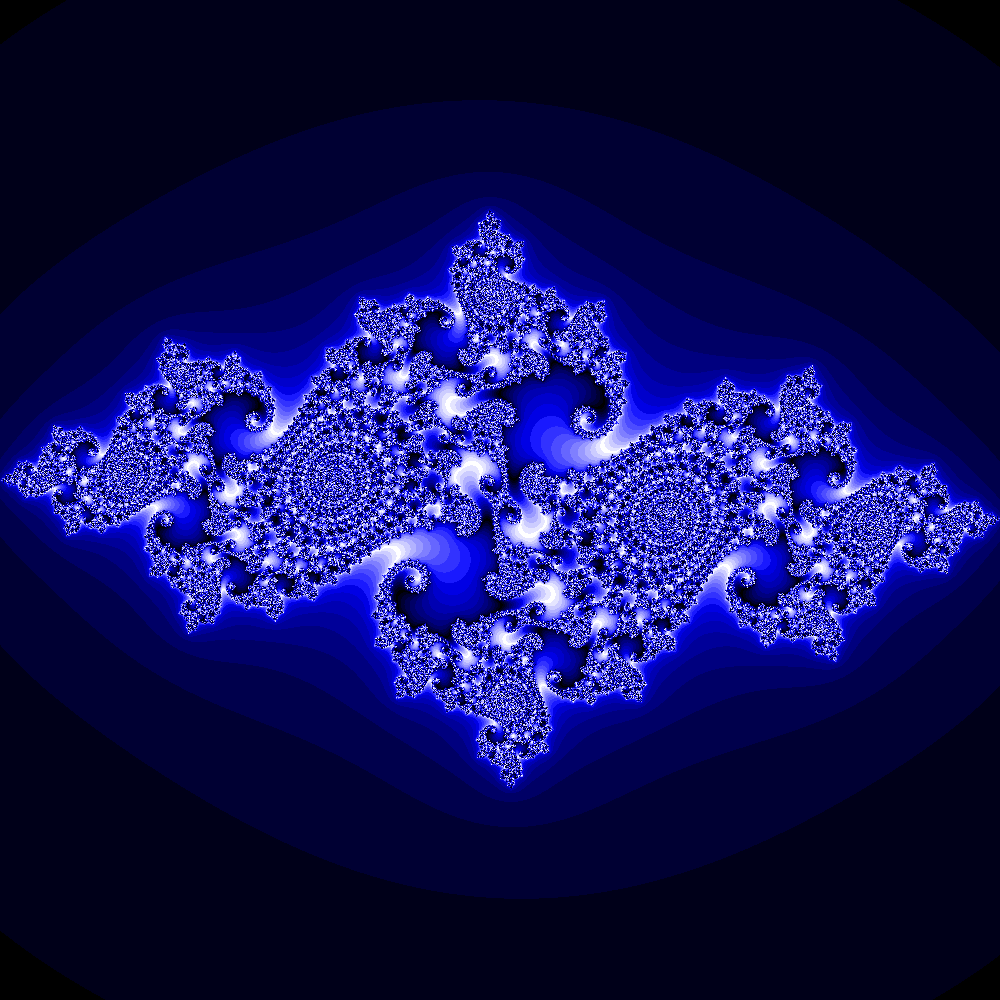
\includegraphics[width=\textwidth]{Julia(5)}
        \caption{K = (0.74543,0.11301)}
        \label{fig:mouse}
    \end{subfigure}
    \caption{Julia Sets}\label{fig:animals}
\end{figure} 

\begin{figure}[!ht]
    \centering
    \begin{subfigure}[h]{0.28\textwidth}
        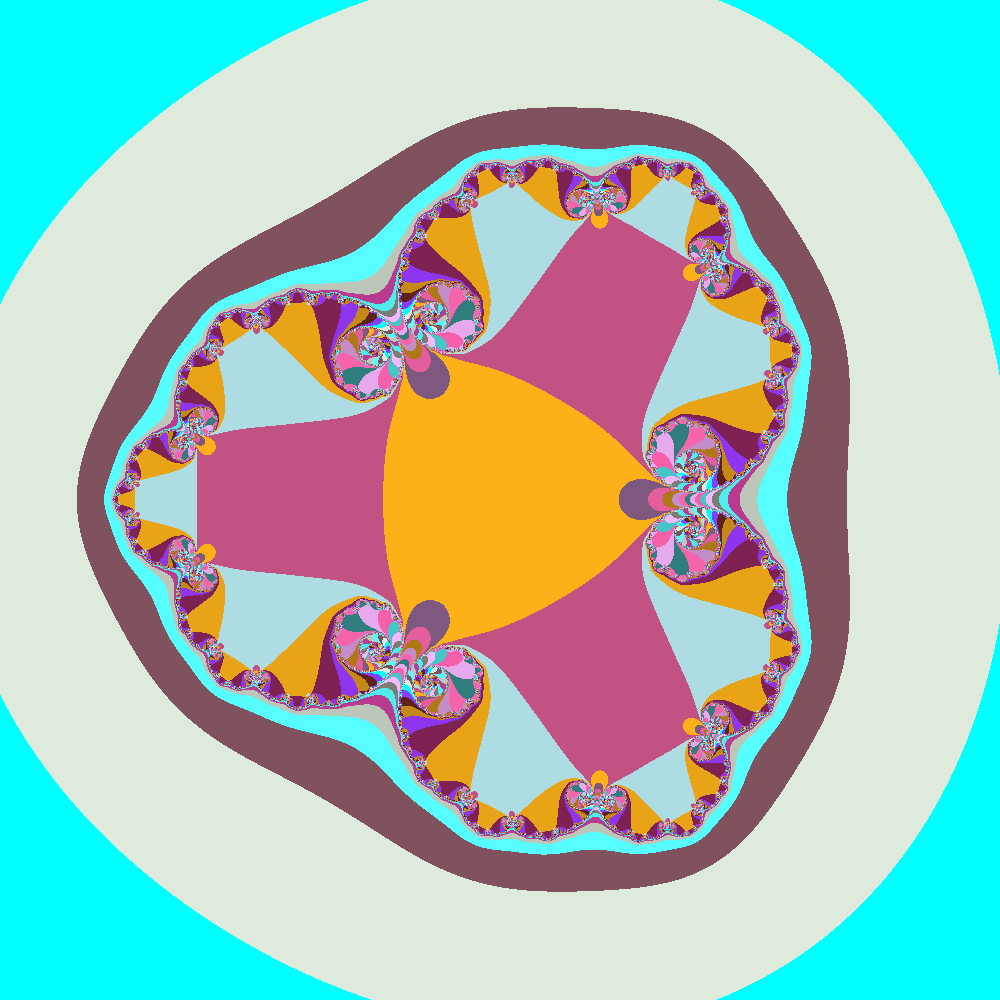
\includegraphics[width=\textwidth]{JuliaCubed}
        \caption{$z^3 + K$ at K = (0.400,0)}
        \label{fig:gull}
    \end{subfigure}%
    ~ %add desired spacing between images, e. g. ~, \quad, \qquad etc.
      %(or a blank line to force the subfigure onto a new line)
    \begin{subfigure}[h]{0.28\textwidth}
        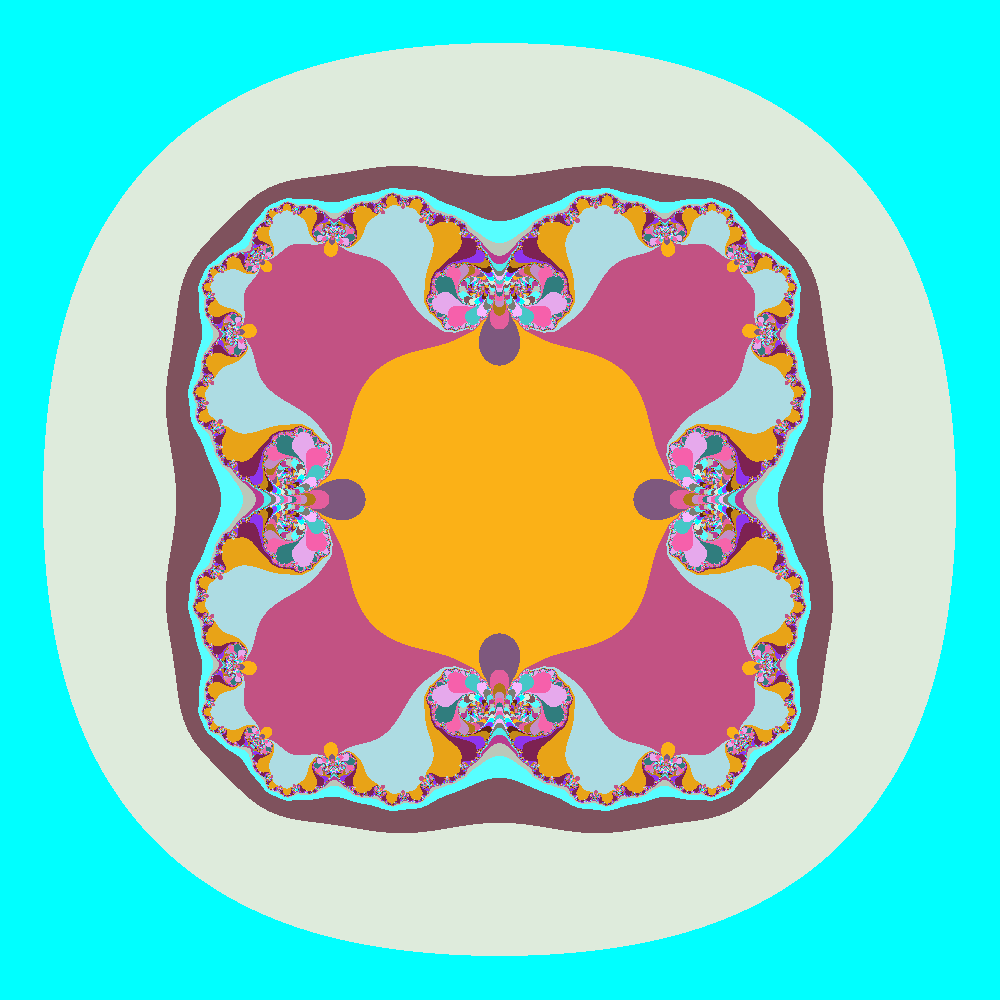
\includegraphics[width=\textwidth]{juliaZFour}
        \caption{$z^4 + K$ at K = (0.484,0)}
        \label{fig:tiger}
    \end{subfigure}
    \begin{subfigure}[h]{0.28\textwidth}
        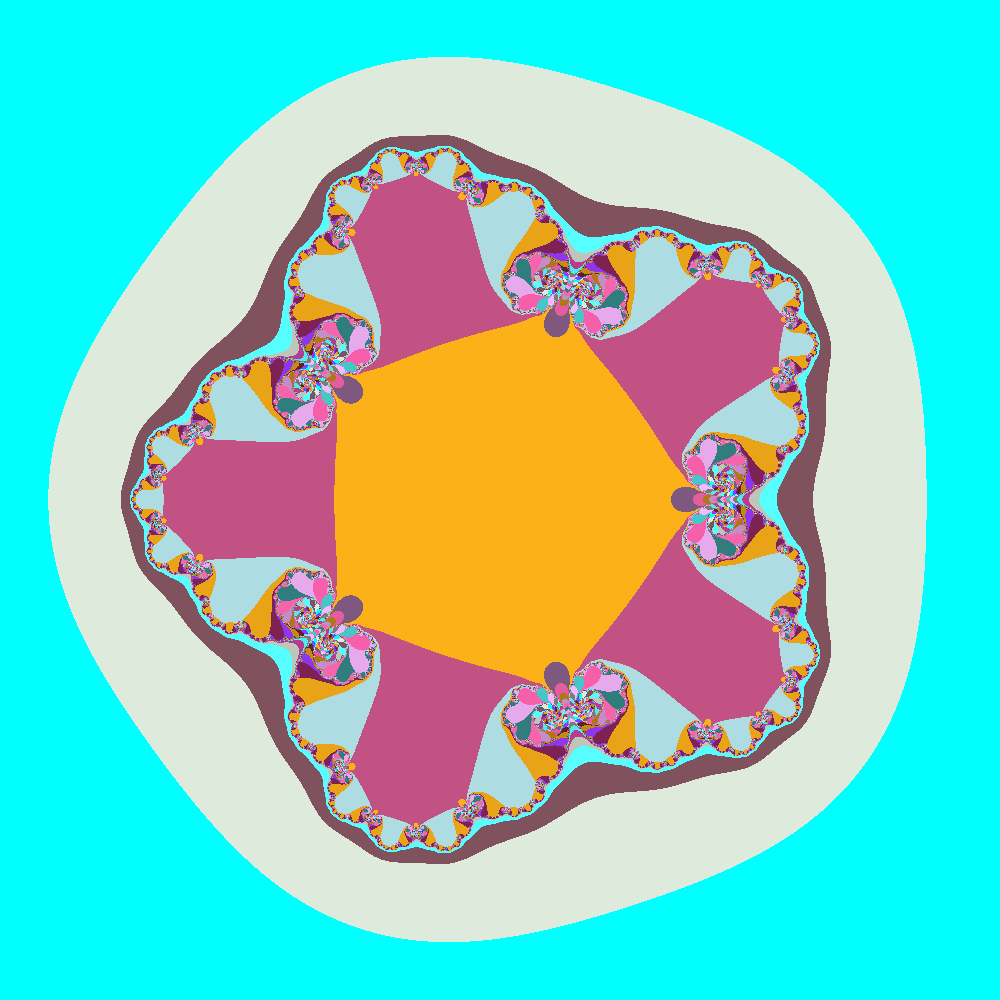
\includegraphics[width=\textwidth]{juliaZFive}
        \caption{$z^5 + K$ at K = (0.544, 0)}
        \label{fig:gull}
    \end{subfigure}%
    ~ %add desired spacing between images, e. g. ~, \quad, \qquad etc.
      %(or a blank line to force the subfigure onto a new line)
    \begin{subfigure}[h]{0.28\textwidth}
        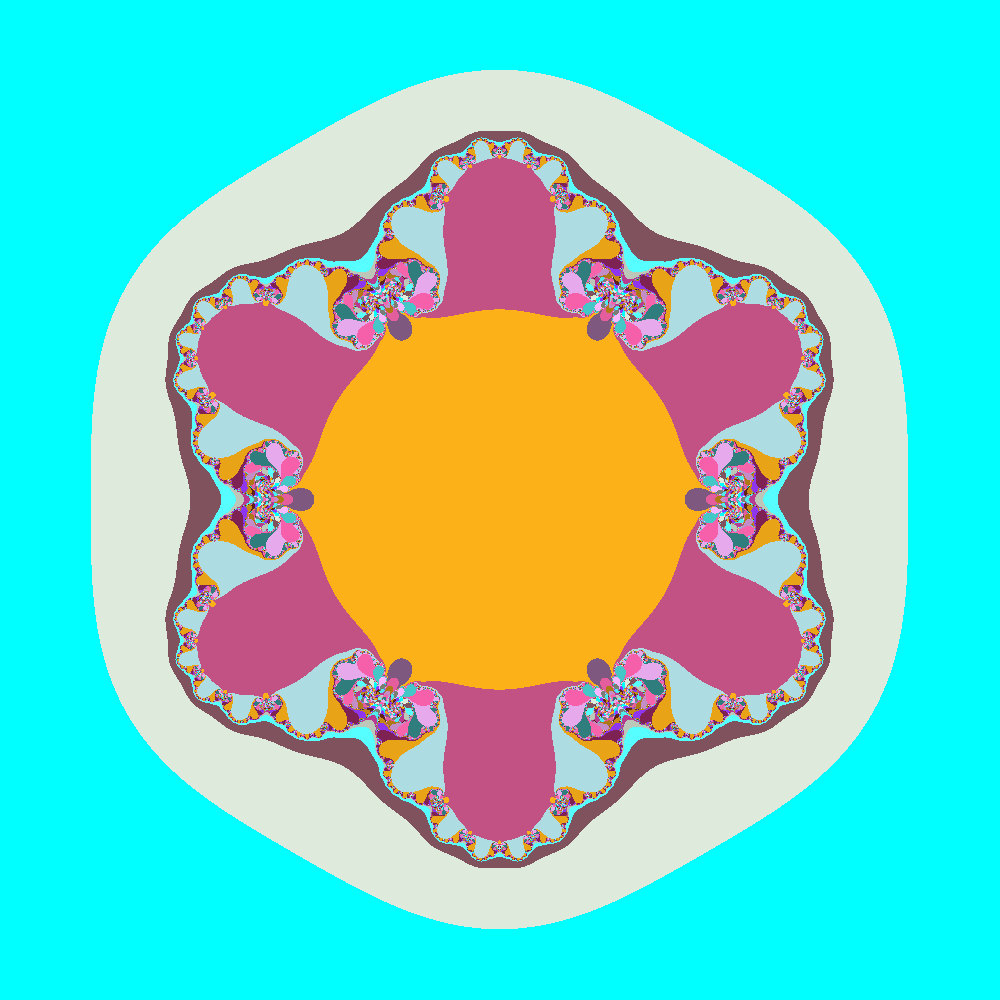
\includegraphics[width=\textwidth]{juliaZSix}
        \caption{$z^6 + K$ at K = (0.590,0)}
        \label{fig:tiger}
    \end{subfigure}
    \caption{Example `monsters'}\label{fig:animals}
\end{figure} 

\section{Benoit Mandelbrot - A Brief History}

In 1958 Mandelbrot joined the giant American corporation IBM, a company pioneering a technology that would soon revolutionise the way we all live - the computer. During his time there he encountered various challenges that would feed his fascination with the visual side of mathematics, which began for him as a student in 1944. 

One problem that Mandelbrot faced at the company was failed transmission in computer data with the use of phone lines. Noticing that every so often the phone lines became noisy, Mandelbrot decided to graph the noise data, and came to the revelation that regardless of the timescale, the plot looked similar. This strange pattern reminded him of what he had seen as a student - a mathematical mystery that dated back nearly a hundred years. 

In the late 19th century, mathematicians had a definition for a curve. However, over time they realised that some of the shapes could satisfy the definition, but were too hard to graph. These shapes were regarded as `monsters' by the mathematicians of this century. 

The first of these ‘monsters’ was created in 1883 by the German mathematician Georg Cantor. He took a straight line, divided it into three equal pieces and removed the middle piece. He repeated the process many times for the lines remaining in the output, as shown in Figure 13(b). As you keep iterating there are infinitely many points left, and this is clear when you zoom into the set of lines. Once you start zooming into the set, it is evident that it has a self-similarity property. This pattern was very similar to the one Mandelbrot had seen at IBM. We also find that the classical H{\'e}non attractor exhibits this same property and magnifying any region of the map will reveal a cantor set structure.

The Swedish mathematician Helge von Koch put forward another strange shape. His process involved taking a small piece from the middle of each side of an equilateral triangle, and replacing each with two slightly longer pieces that formed bumped triangles on each side. Iteration of this method would create an infinitely long curve, and thus a paradox. To the eye the curve looks finite, but mathematically it is infinite. The von Koch snowflake turned out to be crucial to understanding the puzzling measurement problem - the length of a coastline. 

\begin{figure}[h]
    \centering
    \begin{subfigure}[h]{0.3\textwidth}
        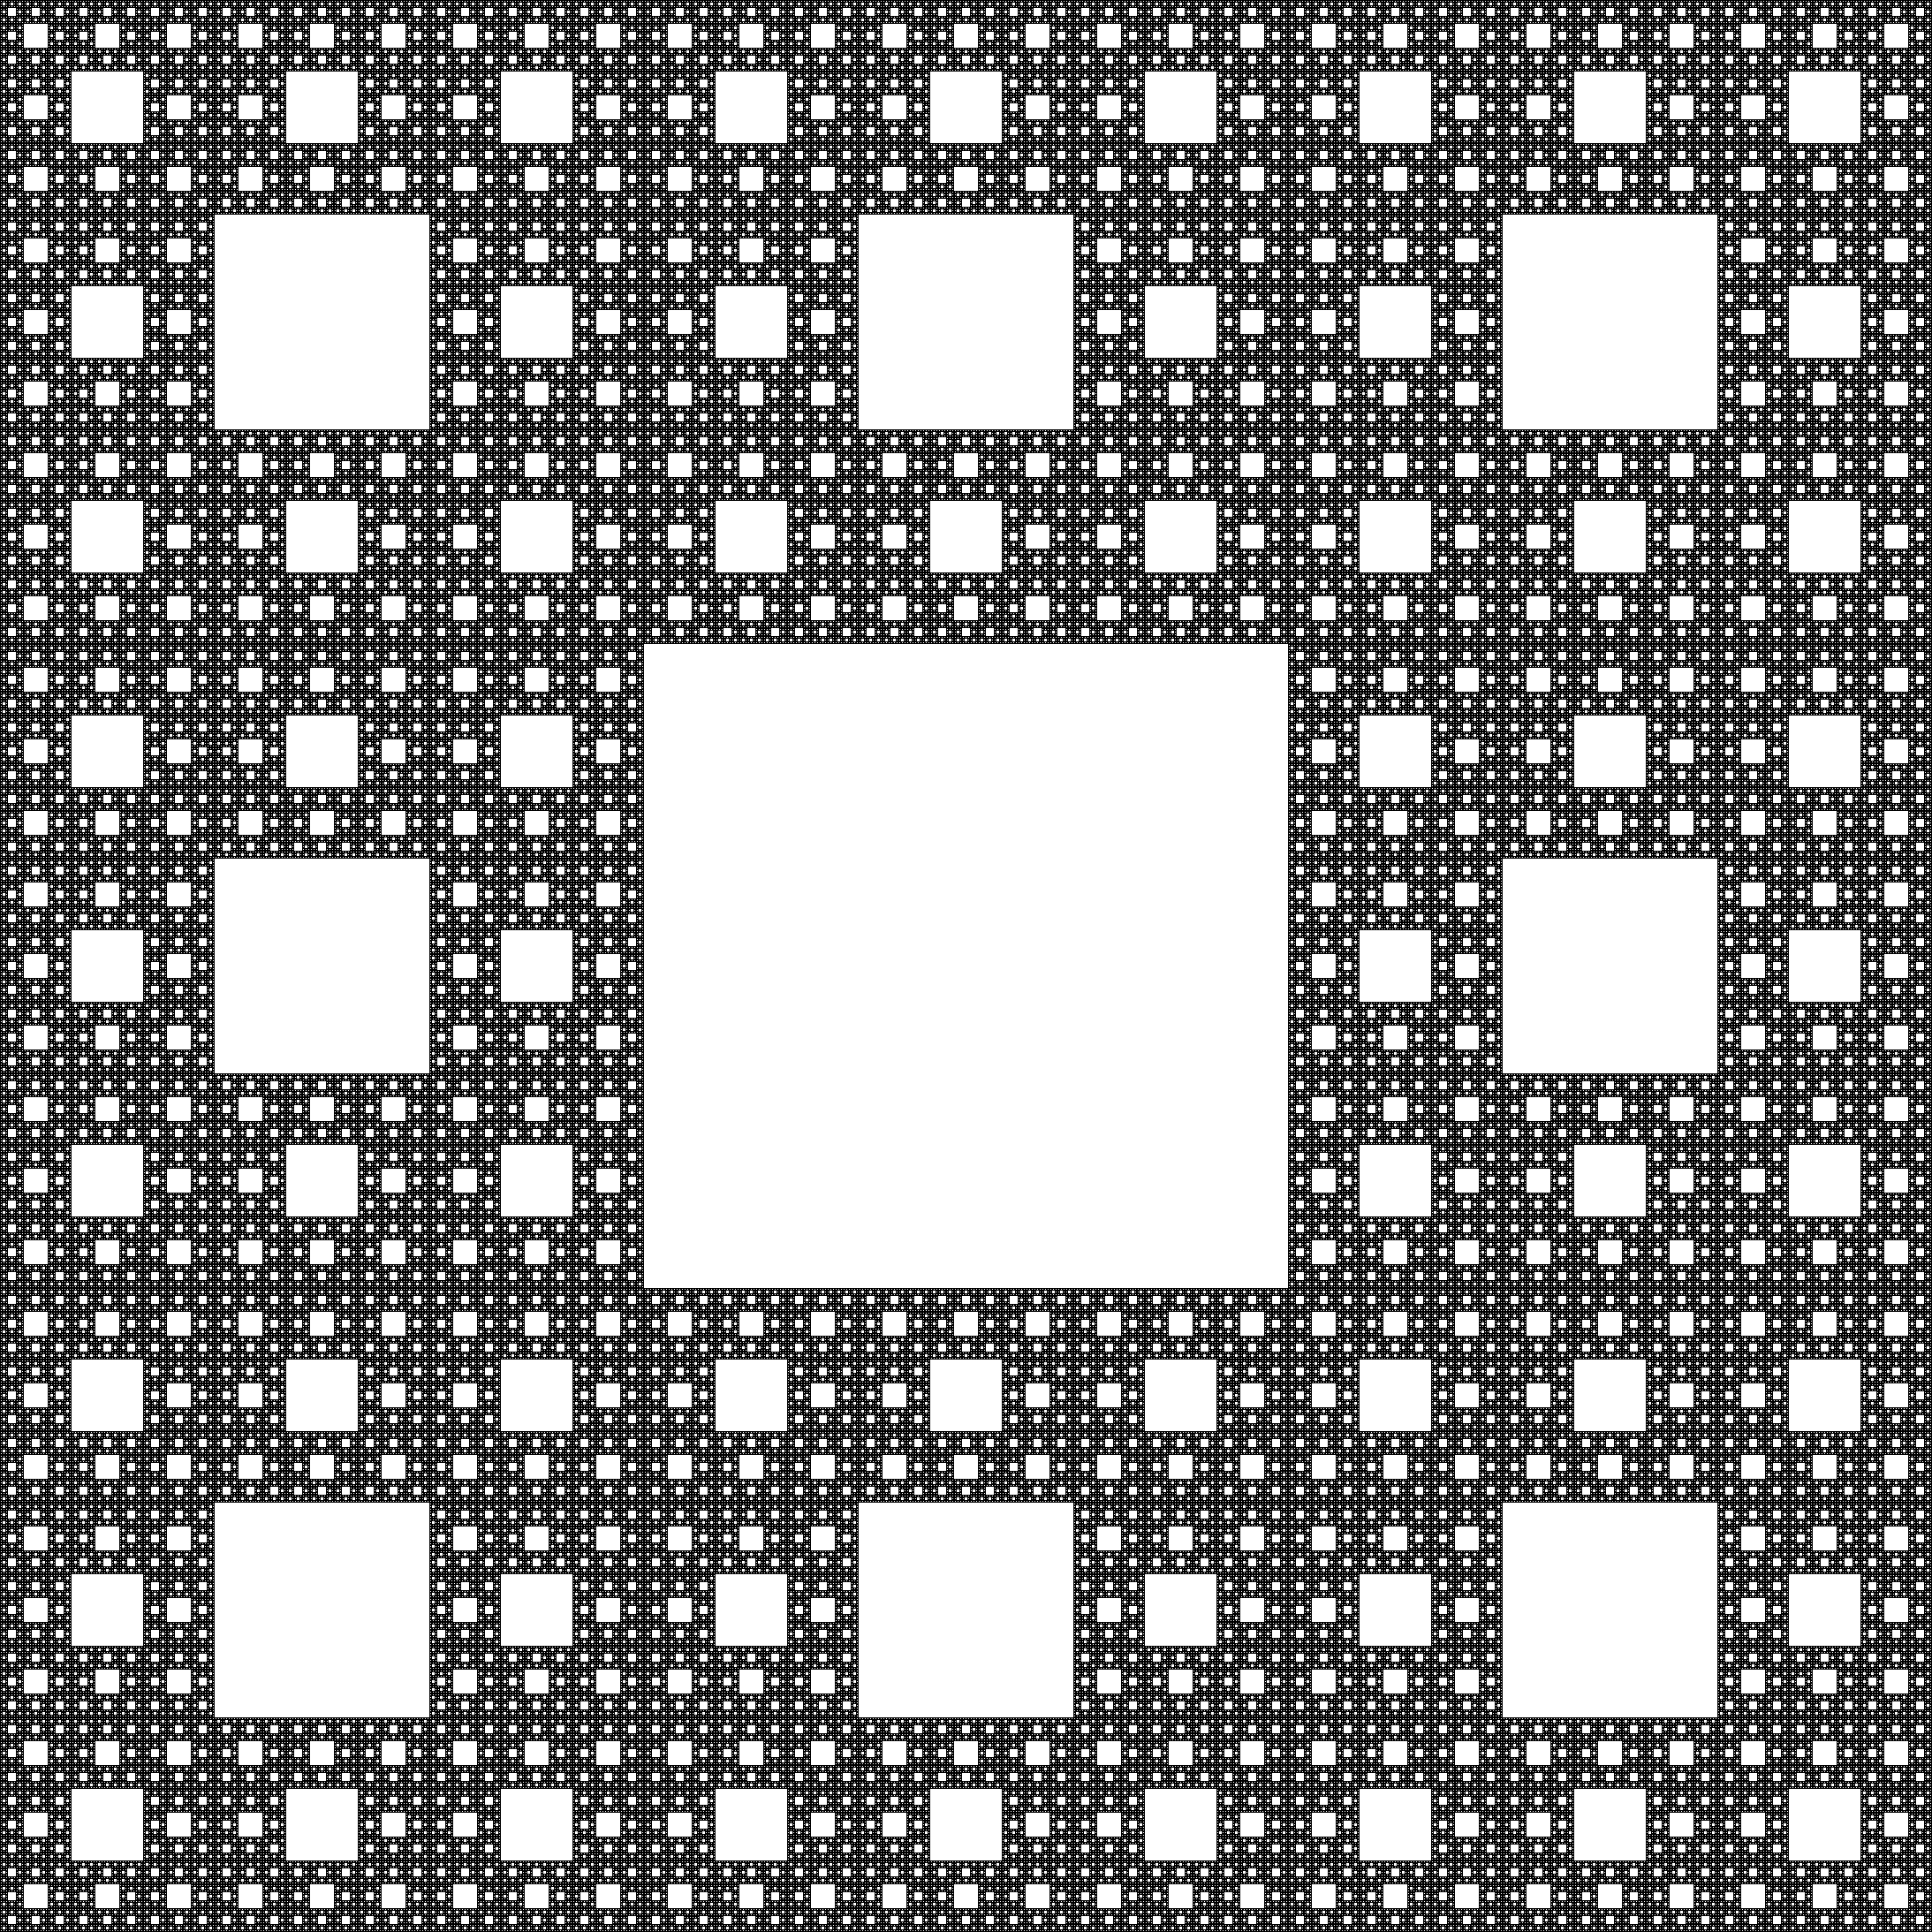
\includegraphics[width=\textwidth]{sierpinski_carpet}
        \caption{Sierpinski Carpet}
        \label{fig:gull}
    \end{subfigure}%
    ~ %add desired spacing between images, e. g. ~, \quad, \qquad etc.
      %(or a blank line to force the subfigure onto a new line)
    \begin{subfigure}[h]{0.3\textwidth}
        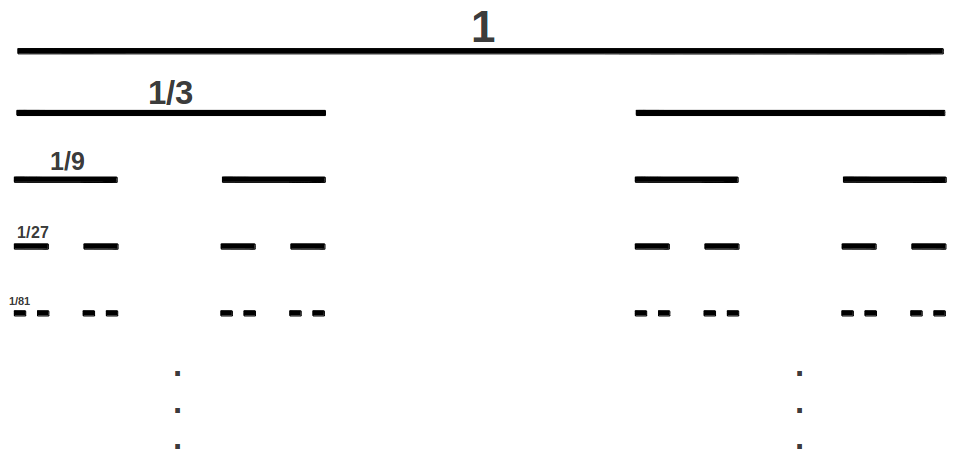
\includegraphics[width=\textwidth]{CantorSet}
        \caption{Cantor Set}
        \label{fig:tiger}
    \end{subfigure}
    ~ %add desired spacing between images, e. g. ~, \quad, \qquad etc.
      %(or a blank line to force the subfigure onto a new line)
    \begin{subfigure}[h]{0.3\textwidth}
        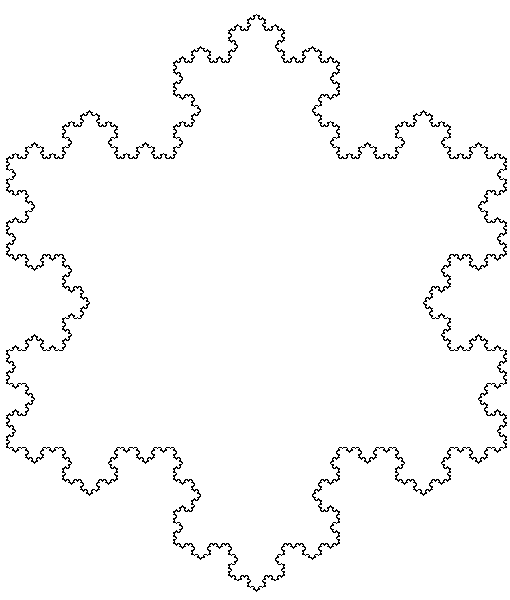
\includegraphics[width=\textwidth]{koch_snowflake}
        \caption{von Koch Snowflake}
        \label{fig:gull}
    \end{subfigure}%
    ~ %add desired spacing between images, e. g. ~, \quad, \qquad etc.
      %(or a blank line to force the subfigure onto a new line)
    \caption{Example `monsters'}\label{fig:animals}
\end{figure} 

In the 1940s, British scientist Lewis Fry Richardson had observed that there are great variations between measurements of a coastline. He was adamant that the length of the measuring instrument was a crucial variable to this variation. A shorter measuring instrument would yield a higher perimeter for the coastline because one would be able to measure finer indentations. Mandelbrot saw a relationship between Richardson’s findings and the von Koch snowflake, and published his thoughts in a famous article in the Science magazine -`How long is the coastline of Britain?'~\cite{Coastline}. A coastline in geometric terms is a fractal, and therefore Mandelbrot opted to measure its roughness instead of its length. However, this piece of analysis required people to rethink one of the basic principles of mathematics - dimension. Mandelbrot reasoned that there were objects whose dimensions are between two and three, and these were called fractals. Furthermore, he stated that there was a positive relationship between roughness and fractal dimension. 

Mandelbrot's enthusiasm for fractals continued to grow, and this inspired him further to explore the work of the French mathematician Gaston Julia. Julia created another one of these strange shapes during WWI, which involved iterating a simple function many times, and plotting the results on a graph. Mandelbrot was able to extend the work done by Julia because of his access to computers, which allowed him to iterate the function extensively. There are infinitely many Julia sets, however, in 1980 Mandelbrot was able to create an equation that combined all of the Julia sets into a single set. The Mandelbrot set was a revolutionary breakthrough, and quickly became famous as the emblem of fractal geometry. 

\begin{thebibliography}{}

\bibitem{Logistic} Paul S. Addison, Fractals and Chaos: An illustrated course, \emph{CRC Press}, 1 Jan 1997 

\bibitem{PeriodDoublingBifurcation} Stephen Lynch, Dynamical Systems with Applications using Mathematica, \emph{Springer Science and Business Media}, 20 Sep 2007

\bibitem{Feigenbaum}Kathleen T. Alligood, Chaos: An Introduction to Dynamical Systems, \emph{Springer Science and Business Media}, 1997

\bibitem{FractalsGraphics} Michael Frame, Benoit Mandelbrot, Fractals, Graphics, and Mathematics Education, \emph{Cambridge University Press}, 20 Jun 2002

\bibitem{FractalsGeometry} Benoit B. Mandelbrot, The Fractal Geometry of Nature, \emph{Henry Holt and Company}, 1983

\bibitem{Klebanoff} Klebanoff, Aaron, $\pi$ in the Mandelbrot Set, 2001 

\bibitem{Bifurcation} Saber N. Elaydi, Discrete Chaos, Second Edition, \emph{CRC Press}, Nov 9, 2007 

\bibitem{piInMandel} Indigestion - finding Pi in the Mandelbrot Set, \emph{Digital Fugue} Jan 01, 2012

\bibitem{Coastline} Benoit Mandelbrot, How Long Is the Coast of Britain?, \emph{Science Mag}, May 5, 1967

\bibitem{IBM History} Benoit Mandelbrot, \emph{The Telegraph} Oct 17, 2010

\end{thebibliography}

\end{document}
\end{document}